%% LyX 1.3 created this file.  For more info, see http://www.lyx.org/.
%% Do not edit unless you really know what you are doing.
\documentclass[english]{article}
\usepackage[T1]{fontenc}
\usepackage[latin1]{inputenc}
\usepackage{a4wide}
\usepackage{color}
\usepackage{graphicx}

\makeatletter

%%%%%%%%%%%%%%%%%%%%%%%%%%%%%% LyX specific LaTeX commands.
\newcommand{\noun}[1]{\textsc{#1}}
%% Because html converters don't know tabularnewline
\providecommand{\tabularnewline}{\\}

%%%%%%%%%%%%%%%%%%%%%%%%%%%%%% Textclass specific LaTeX commands.
 \newenvironment{lyxcode}
   {\begin{list}{}{
     \setlength{\rightmargin}{\leftmargin}
     \setlength{\listparindent}{0pt}% needed for AMS classes
     \raggedright
     \setlength{\itemsep}{0pt}
     \setlength{\parsep}{0pt}
     \normalfont\ttfamily}%
    \item[]}
   {\end{list}}

\AtBeginDocument{
  \renewcommand{\labelitemi}{\(\cdot\)}
}

\usepackage{babel}
\makeatother
\begin{document}

\title{The Reliable Multicast Library (RML) and Tangram II Whiteboard Developer
Documentation}


\author{Jorge Allyson Azevedo, Milena Scanferla, Daniel Sadoc\\
\{allyson,milena,sadoc\}@land.ufrj.br}

\maketitle

\section{Introduction}

The main goal of this article is to explain some topics about what
a programmer needs to know in order to make source code changes in
the Reliable Multicast Library (RML) and in the Tangram II Whiteboard.
We will also give comments about problems found and the solutions
adopted while developing the RML and the Tangram II \cite{key-30}
Whiteboard tool - including references to books, newsgroups or articles
that may be useful for the interested readers. In the following section
we will take a look at general characteristics of IP multicast. Then,
the reliable multicast approach used in the implemented RML will be
describe. We will introduce the library, and show a sample program
that makes use of it - a chat. After that, a more complex example
- the Tangram II Whiteboard (TGWB). In the Appendix, we will describe
the operating system interprocess communication (IPC) resources that
which have been used.

%
\begin{figure}[hbpt]
\begin{center}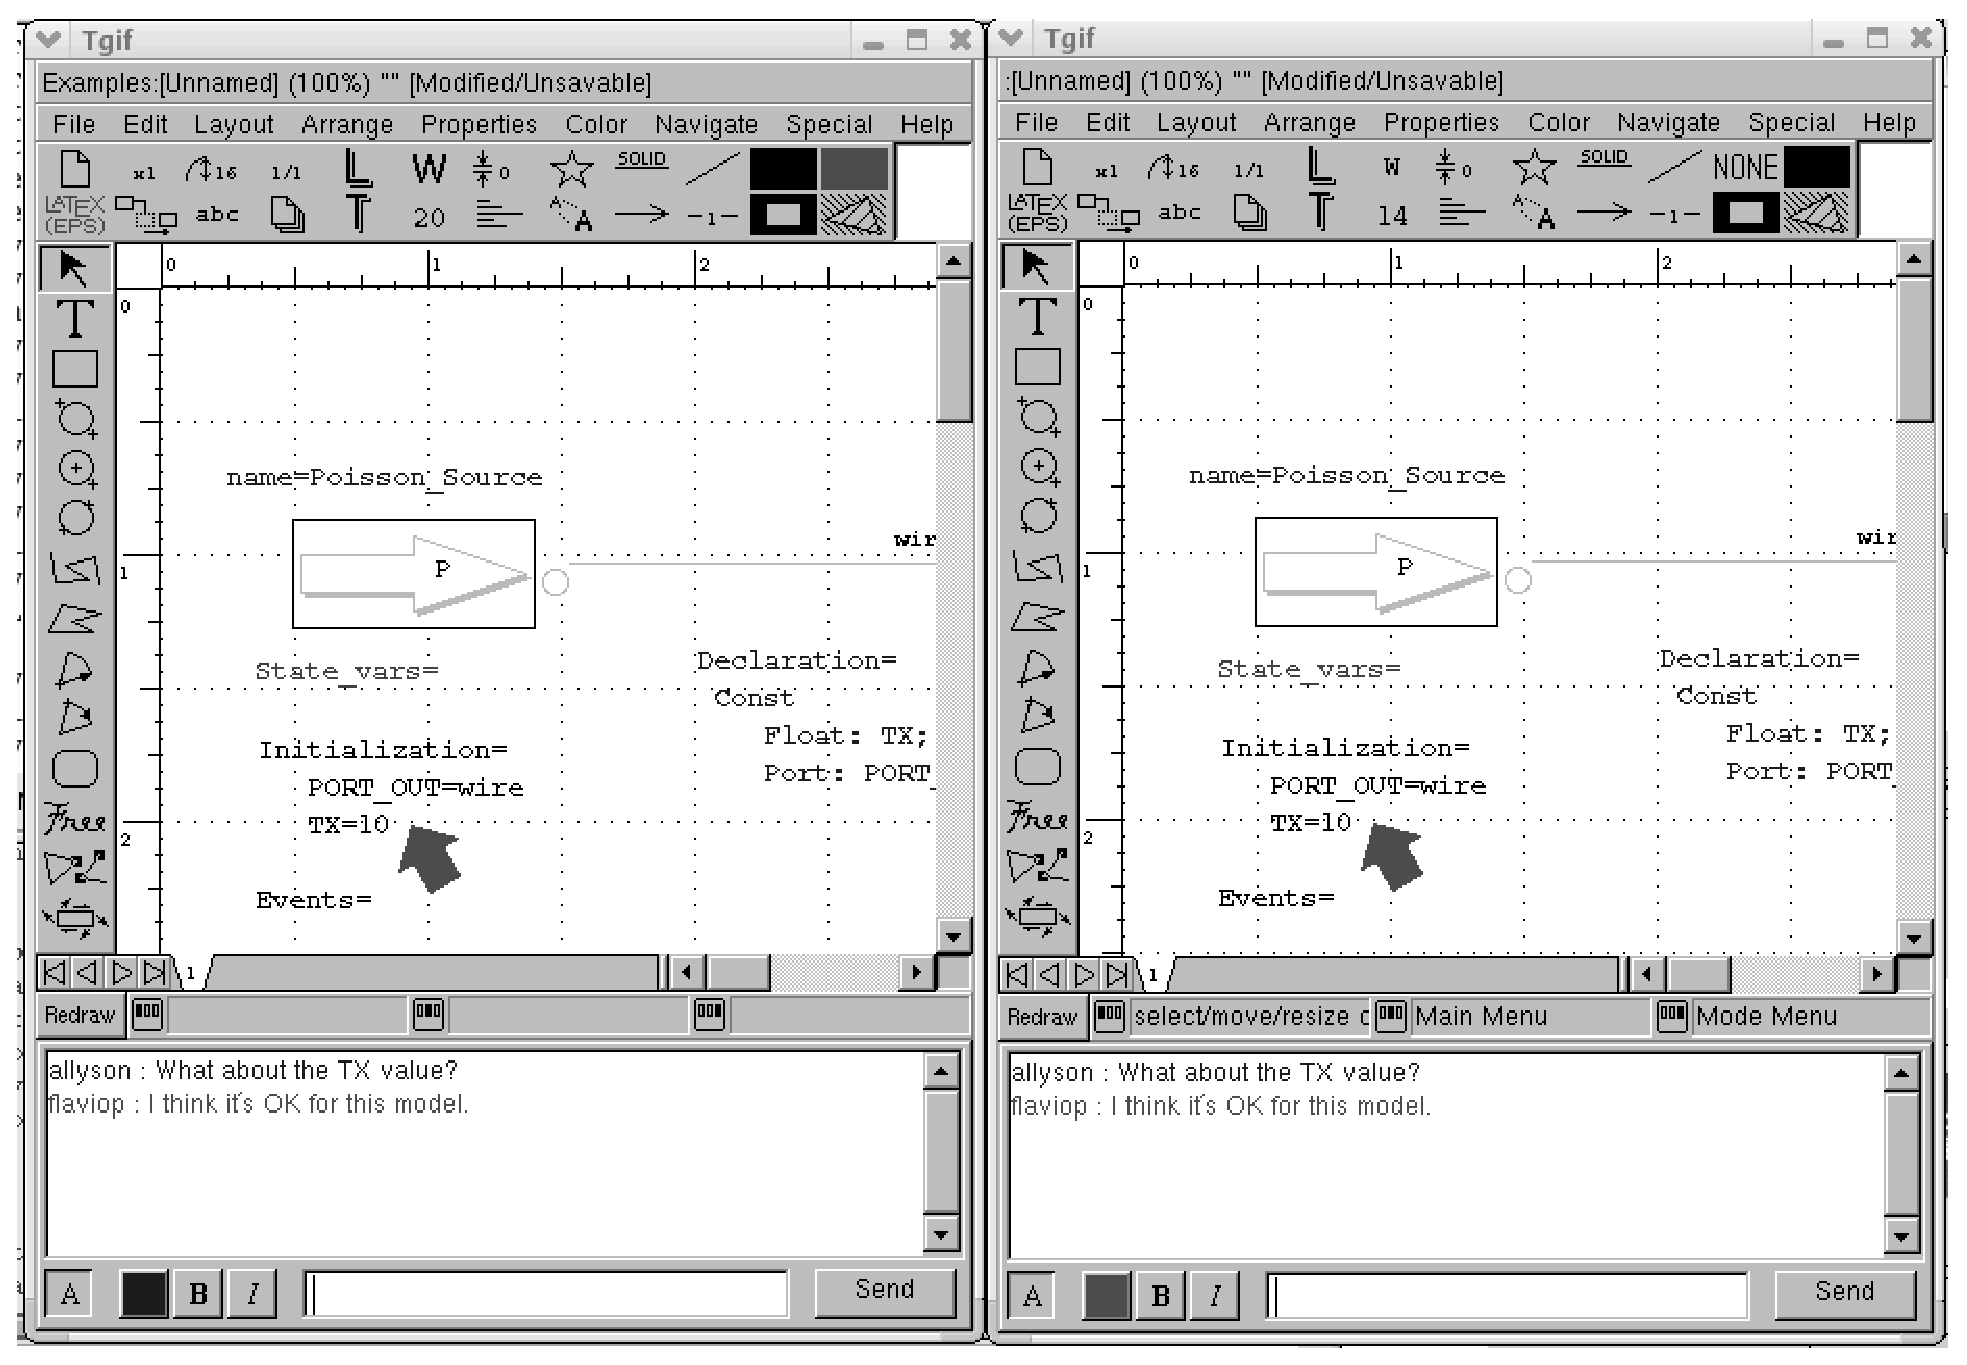
\includegraphics[%
  width=1.0\columnwidth]{screencapt.eps}\end{center}


\caption{TGWB Screenshot}
\end{figure}



\section{IP Multicast }


\subsection{Introduction}

Quoting from the Multicast HOWTO \cite{key-33}: {}``... multicast
is a need ... Well, at least in some scenarios. If you have information
(a lot of information, usually) that should be transmitted to various
(but usually not all) hosts over an internet, then Multicast is the
answer. One common situation in which it is used is when distributing
real time audio and video to the set of hosts which have joined a
distributed conference. 

Multicast is much like radio or TV in the sense that only those who
have tuned their receivers (by selecting a particular frequency they
are interested on) receive the information. That is: you hear the
channel you are interested in, but not the others.''


\subsubsection{Multicast Addressing}

The range of IP addresses is divided into \char`\"{}classes\char`\"{}
based on the high order bits of a 32 bits IP address: \\


\texttt{\textit{\textcolor{black}{0~~~~~~~~~~~~~~~~~~~~~~~~~~
31~~~~~~~~~ Address Range:}}}

\texttt{\textit{\textcolor{black}{+-+-{}-{}-{}-{}-{}-{}-{}-{}-{}-{}-{}-{}-{}-{}-{}-{}-{}-{}-{}-{}-{}-{}-{}-{}-{}-{}-{}-+}}}

\texttt{\textit{\textcolor{black}{|0|~~~~~~ Class A Address~~~~~
|~~~~ 0.0.0.0 - 127.255.255.255}}}

\texttt{\textit{\textcolor{black}{+-+-{}-{}-{}-{}-{}-{}-{}-{}-{}-{}-{}-{}-{}-{}-{}-{}-{}-{}-{}-{}-{}-{}-{}-{}-{}-{}-{}-+}}}

\texttt{\textit{\textcolor{black}{+-+-+-{}-{}-{}-{}-{}-{}-{}-{}-{}-{}-{}-{}-{}-{}-{}-{}-{}-{}-{}-{}-{}-{}-{}-{}-{}-+}}}

\texttt{\textit{\textcolor{black}{|1 0|~~~~ Class B Address~~~~~
|~~ 128.0.0.0 - 191.255.255.255}}}

\texttt{\textit{\textcolor{black}{+-+-+-{}-{}-{}-{}-{}-{}-{}-{}-{}-{}-{}-{}-{}-{}-{}-{}-{}-{}-{}-{}-{}-{}-{}-{}-{}-+}}}

\texttt{\textit{\textcolor{black}{+-+-+-+-{}-{}-{}-{}-{}-{}-{}-{}-{}-{}-{}-{}-{}-{}-{}-{}-{}-{}-{}-{}-{}-{}-{}-+}}}

\texttt{\textit{\textcolor{black}{|1 1 0|~~ Class C Address~~~~~
|~~ 192.0.0.0 - 223.255.255.255}}}

\texttt{\textit{\textcolor{black}{+-+-+-+-{}-{}-{}-{}-{}-{}-{}-{}-{}-{}-{}-{}-{}-{}-{}-{}-{}-{}-{}-{}-{}-{}-{}-+}}}

\texttt{\textit{\textcolor{black}{+-+-+-+-+-{}-{}-{}-{}-{}-{}-{}-{}-{}-{}-{}-{}-{}-{}-{}-{}-{}-{}-{}-{}-{}-+}}}

\texttt{\textit{\textcolor{black}{|1 1 1 0|~ MULTICAST Address~~
|~~ 224.0.0.0 - 239.255.255.255}}}

\texttt{\textit{\textcolor{black}{+-+-+-+-+-{}-{}-{}-{}-{}-{}-{}-{}-{}-{}-{}-{}-{}-{}-{}-{}-{}-{}-{}-{}-{}-+}}}

\texttt{\textit{\textcolor{black}{+-+-+-+-+-+-{}-{}-{}-{}-{}-{}-{}-{}-{}-{}-{}-{}-{}-{}-{}-{}-{}-{}-{}-+}}}

\texttt{\textit{\textcolor{black}{|1 1 1 1 0|~~~~ Reserved~~~~~~
|~~ 240.0.0.0 - 247.255.255.255}}}

\texttt{\textit{\textcolor{black}{+-+-+-+-+-+-{}-{}-{}-{}-{}-{}-{}-{}-{}-{}-{}-{}-{}-{}-{}-{}-{}-{}-{}-+}}}~\\


The multicast addresses start with {}``1110''. Among the multicast
addresses, the remaining 28 bits identify the multicast group. There
are some special addresses that should not be used by common applications:

%
\begin{table}[hbpt]
\begin{center}\begin{tabular}{|c|c|}
\hline 
Address&
Function\tabularnewline
\hline
\hline 
224.0.0.1&
All hosts in the LAN\tabularnewline
\hline 
224.0.0.2&
All routers in the LAN\tabularnewline
\hline 
224.0.0.4&
All routers DVMRP in the LAN\tabularnewline
\hline 
224.0.0.5&
All routers OSPF in the LAN\tabularnewline
\hline 
224.0.0.6&
All routers OSPF designated in the LAN\tabularnewline
\hline 
224.0.0.13&
All the PIM routers in the LAN\tabularnewline
\hline
\end{tabular}\end{center}


\caption{\label{mcast special addresses}Multicast special addresses}
\end{table}
The interval from 224.0.0.0 to 224.0.0.255 is reserved to local purposes
(local administrative tasks) - to see some of these address purposes,
refer to table \ref{mcast special addresses}. Similarly, the interval
from 239.0.0.0 to 239.255.255.255 is also reserved for administrative
tasks - but not necessarily local tasks. So, the interval that may
be used by general multicast applications is from 225.0.0.0 to 238.255.255.255.


\subsubsection{Multicast Group}

A multicast group is composed by the set of hosts in a network which
share data via multicast. This group is identified by a multicast
address. When a host sends a packet to the multicast address, this
packet is received by all the multicast group members. The transmission
of a packet from one sender to multiple receivers is accomplished
by a single send operation. A single packet is sent from the sender
host - there is no need to send multiple copies of this packet, as
would be needed if unicast were used.

The receivers may join and leave the multicast group in a dynamic
way. The network devices, specially the routers, have to determine
which of their interfaces have a multicast member connected to them.


\subsubsection{Levels of conformance}

Hosts can be in three different levels of conformance with the Multicast
specification, according to the requirements they meet: 

\begin{itemize}
\item \textbf{Level 0} is the \char`\"{}no support for IP Multicasting\char`\"{}
level. Lots of hosts and routers in the Internet are in this state,
as multicast support is not mandatory in IPv4 (it is, however, in
IPv6). Not too much explanation is needed here: hosts in this level
can neither send nor receive multicast packets. They must ignore the
ones sent by other multicast hosts. 
\item \textbf{Level 1} is the \char`\"{}support for sending but not receiving
multicast IP datagrams\char`\"{} level. Thus, note that it is not
necessary to join a multicast group to be able to send datagrams to
it. Very few additions are needed in the IP module to make a \char`\"{}Level
0\char`\"{} host \char`\"{}Level 1-compliant\char`\"{}. 
\item \textbf{Level 2} is the \char`\"{}full support for IP multicasting\char`\"{}
level. Level 2 hosts must be able to both send and receive multicast
traffic. They must know the way to join and leave multicast groups
and to propagate this information to multicast routers. Thus, they
must include an Internet Group Management Protocol (IGMP) implementation
in their TCP/IP stack.
\end{itemize}
The Multicast Reliable Library was developed considering that the
hosts are in level 2 of conformance. 


\subsubsection{Some benefits of Multicast}

Some benefits of multicast over unicast are presented below\cite{key-35}:

\begin{enumerate}
\item Optimized use of the network - the intelligent use of the network
resources avoids unnecessary replication of data. So, the links are
better used, through a better architecture of data distribution.
\item Distributed application support - the multicast technology is directly
focused on distributed applications. Multimedia applications like
distance learning and video conferencing may be used in the network
in an efficient way. 
\item Scalability - services that use multicast can be accessed by many
hosts, and may accept new members at any time.
\item Availability of the network resources - congestion is reduced, because
no replicated data is sent through a single link in the network, so
the availability of the network resources is increased.
\end{enumerate}

\subsection{Configuration under Linux }

This section will not explain multicast configuration in details.
We just want to give some tips needed to set up a basic system in
a local network area. If you want further information see the Multicast
HOWTO \cite{key-33}. Multicast transmission through different networks
is more complex and you must have routers with multicast support between
those networks. 


\subsubsection{Does your system have support for IP Multicast? }

Some configurations are needed to use IP Multicast. First of all,
the network cards have to be enabled to receive multicast data. Most
network cards modules automatically set the MULTICAST flag. In GNU/Linux
systems, you can check whether your network interface has multicast
support by typing the following command:

\begin{quotation}
\texttt{\footnotesize ifconfig -a}{\footnotesize \par}
\end{quotation}
An ifconfig output example follows:

\begin{verse}
\texttt{\footnotesize eth0 }{\footnotesize \par}

\texttt{\footnotesize Link encap:Ethernet HWaddr 00:50:BF:06:89:47}~\\
\texttt{\footnotesize inet addr:192.168.1.2 Bcast:192.168.1.255 Mask:255.255.255.0
}~\\
\texttt{\footnotesize UP BROADCAST RUNNING} \texttt{\textbf{\footnotesize MULTICAST}}
\texttt{\footnotesize MTU:1500 Metric:1 }~\\
\texttt{\footnotesize RX packets:12438583 errors:0 dropped:0 overruns:0
frame:0 }~\\
\texttt{\footnotesize TX packets:6498370 errors:0 dropped:0 overruns:0
carrier:0 }~\\
\texttt{\footnotesize collisions:0 txqueuelen:100 }~\\
\texttt{\footnotesize RX bytes:1100375580 (1049.3 Mb) }~\\
\texttt{\footnotesize TX bytes:2158372342 (2058.3 Mb) }~\\
\texttt{\footnotesize Interrupt:10 Base address:0x7000}{\footnotesize \par}

\texttt{\footnotesize lo }{\footnotesize \par}

\texttt{\footnotesize Link encap:Local Loopback }~\\
\texttt{\footnotesize inet addr:127.0.0.1 Mask:255.0.0.0 }~\\
\texttt{\footnotesize UP LOOPBACK RUNNING MTU:16436 Metric:1 }~\\
\texttt{\footnotesize RX packets:8361666 errors:0 dropped:0 overruns:0
frame:0 }~\\
\texttt{\footnotesize TX packets:8361666 errors:0 dropped:0 overruns:0
carrier:0 }~\\
\texttt{\footnotesize collisions:0 txqueuelen:0 }~\\
\texttt{\footnotesize RX bytes:1830657956 (1745.8 Mb) }~\\
\texttt{\footnotesize TX bytes:1830657956 (1745.8 Mb)}{\footnotesize \par}
\end{verse}
Note the MULTICAST flag at \textbf{eth0}. That flag is missed at \textbf{lo}
(the loopback interface). You must have root privileges to enable
the MULTICAST flag. To enable that flag you have to issue the following
command:

\begin{verse}
\texttt{\footnotesize ifconfig <interface\_name> multicast}{\footnotesize \par}
\end{verse}
Where \textbf{interface\_name} must be replaced by the name of the
interface you want to set the MULTICAST flag. This may be useful if
you want to enable multicast on a \textbf{lo} interface because that
allows you to do some tests using multicast transmission even if you
don't have any real network interface. The next step is to set up
the route that the multicast packets will follow. To add this route,
as root user, issue the following command:

\begin{verse}
\texttt{\footnotesize route add -net 224.0.0.0 netmask 240.0.0.0 dev
<interface\_name>}{\footnotesize \par}
\end{verse}
Where \textbf{interface\_name} must be replaced by the name of the
interface to which you want to send the multicast packets. Again,
if you are testing on a single machine this interface will be the
\textbf{lo.} To test your configuration try:

\begin{verse}
\texttt{\footnotesize ping 224.0.0.1}{\footnotesize \par}
\end{verse}
Every machine in your local network that has multicast enabled should
answer this ping.


\section{Reliable Multicast }


\subsection{Introduction}

Multicast is supported by the transport layer through the UDP protocol.
As each packet may get a different path from source to destiny, packets
may come out of order at the receiver host. To solve this problem,
it is necessary to have a packet ordering algorithm. Besides the problem
of ordering, there is also the possibility of packet loss. This loss
makes the protocol unreliable. To solve these problems, which are
directly related to the UDP protocol, it is necessary to create an
application-level mechanism to guarantee the reliable transmission
of data. 

There are some ways to implement the reliable multicast mechanism.
For instance, the responsibility of recovering loss packets can be
directed to the receiver or the sender of the data. 

Here, we will describe three classes of reliable multicast protocols,
according to {[}FIXME{]}:

\begin{enumerate}
\item Sender Initiated Approach - based on confirmations (acknowledgments
or ACKs) sent by receivers and processed by the senders;
\item Receiver Initiated Approach - the receiver detects the loss of packets.
The receiver sends negative acknowledgments (NACKs) to the sender
via a unicast connection. The sender replies with retransmissions.
\item Enhanced Receiver Initiated Approach - the receiver detects the loss
of packets. The receiver sends negative acknowledgments (NACKs) to
the group via a multicast connection.
\end{enumerate}

\subsubsection{Sender Initiated Approach}

Every time a member receives a packet he sends a confirmation (ACK)
to the sender. The sender maintains a list of all the group members.
When the sender sends a packet, he starts a timer for that packet,
and waits for ACKs from the group members. As soon as the timer expires,
if the sender haven't received an ACK from some member, this packet
is retransmitted. The timer is then restarted.


\subsubsection*{Advantages and disadvantages}

The main advantage of this approach is that when the sender receives
a confirmation (ACK), he is sure that the packet was in fact received.
The main disadvantage of this approach is that for each data packet
sent, the sender will receive an ACK from each receiver of the multicast
session, which may cause congestion. 


\subsubsection*{Summary}

\begin{enumerate}
\item every time the sender transmits or retransmits a data packet he starts
a timer for this packet and wait for the ACKs from the receivers;
\item every time the receiver receives a data packet he sends a confirmation
(ACK) to the sender in a unicast connection.
\end{enumerate}

\subsubsection{Receiver Initiated Approach}

In this approach, the receiver has the responsibility of detecting
the packet losses. When the receiver doesn't receive a data packet,
he sends a negative acknowledgment (NACK) to the sender, via a unicast
connection. The sender will retransmit the data packet when he receives
a NACK. 

The packet loss is detected when a receiver receives a packet with
sequence number (sn) i + 1 without having received the packet with
sn i. For instance, if the receiver receives packets with sn 0, 1
and 3, he will know that packet with sn 2 was lost.


\subsubsection*{Advantages and disadvantages}

In general, the loss probability of a packet is smaller than the success
probability. So, few NACK packets will be sent through the network.
The disadvantage of this approach is that just the sender of the message
will be notified that a packet was lost, and only he may retransmit
the data packet.


\subsubsection*{Summary}

\begin{enumerate}
\item every time the receiver detects a packet loss he sends a negative
acknowledgment (NACK) to the sender, via a unicast connection, and
starts a timer to wait for a retransmission.
\item every time the sender receives a NACK packet he sends a retransmission
to the group via multicast connection.
\end{enumerate}

\subsubsection{Enhanced Receiver Initiated Approach}

That's a variation of the receiver initiated approach. When a loss
is detected, a timer is scheduled. If the timer expires and a NACK
for that packet has not been received, the receiver multicasts the
request message to the group. If a NACK was received before the timer
has expired, the receiver will not send the request message, because
he knows that a retransmission request has already been sent by some
other member.


\subsubsection*{Advantages and disadvantages}

The advantage of this approach is that it limits the number of NACKs
which will be sent through the network. The disadvantage is that when
the loss probability is high, there will be many NACK packets in the
network. Each member of the group will receive all the NACKs sent.
This may consume a lot of processing time. 


\subsubsection*{Summary}

\begin{enumerate}
\item every time the receiver detects a packet loss, he starts a timer to
send a NACK packet. 

\begin{enumerate}
\item If he receives a NACK for the same packet which was lost, the transmission
of the NACK is canceled (NACK suppression). 
\item Else, when the timer expires, he sends a NACK via multicast to the
group.\\
\\
In both cases, another timer is started, in order to wait for retransmissions.
If a retransmission is received, this timer is canceled, and there
is nothing else to be done. The data was finally successfully received
with success. Else, the timer to send a NACK packet is restarted.
We go back to item 1.
\end{enumerate}
\item every time a member receives a NACK packet, he schedules the retransmission
of the requested packet.
\end{enumerate}

\section{The Reliable Multicast Library (RML)}

In this section we will describe how the Reliable Multicast Library
works. In section 4.1, definitions will be given. In section 4.2 the
mechanisms of how new members join and leave the group will be explained.
Then, we will describe how lost packets are recovered in section 4.3.
In section 4.4 we show the implementation of the Event List. Finally,
we summarize the RML messages and actions in section 4.5.


\subsection{Definitions}

Before starting the description of the RML protocol, it is important
to define some terms that will be used:

\begin{itemize}
\item \textbf{Multicast Session}: a multicast session is the period of time
when a multicast group is active. A multicast group is active if we
have at least one member on it.
\item \textbf{ACK}: a special packet, the acknowledgment (ACK) packet, is
used to confirm the receiving of data. For instance, in the TCP protocol,
the sender always waits for confirmations sent by the receivers via
ACKs.
\item \textbf{NACK}: a special packet, the negative acknowledgment (NACK)
packet, is used to inform that data was lost. If a receiver finds
out that data was lost, he may send NACKs to the sender in order to
advertise this problem, and request retransmissions.
\item \textbf{Timers}: the time that a member waits in order to execute
a specific action (event). This time may be random, with an uniform
or exponential distribution.
\item \textbf{Event List}: list containing all the events that will be executed.
When the timer for a specific event expires, this event is removed
from the event list and then executed.
\item \textbf{Cache:} structure maintained by the multicast members which
stores the last messages received from every member of the multicast
session.
\end{itemize}

\subsection{Multicast Session Members Management}

May anyone join a multicast session at any time? What does a new member
need to get in order to become a member of a multicast session? What
about the exit procedure? If a member wants to leave the group, may
he go away immediately? Or should he wait a bit before exiting? This
section will answer this questions.

Let's start with the join procedure. If every member of the multicast
group entered the session always at the same time, the join procedure
would be very simple. The problem is that, in practice, a new member
may want to join the session a long time after the session has started.
If that happens, this member may not be able to get into a consistent
state just requesting retransmissions to the older members of the
group. That's because the size of the cache of the other members of
the group is finite. The data requested by the new member may not
be any more in the cache of the older members.

During a session, each member maintains a certain quantity of data
in his own cache. When this cache gets full, new data replaces the
oldest. If a new member enters the group a long time after the session
has started, it may happen that he won't be able to receive the older
data, since it has been replaced in all the current members caches.

For some applications, that may not be a problem. But for drawing
applications, such as the TGWB, in which there is a dependency between
the data, this problem must be regarded with attention. For instance,
the first message received by a member, in a drawing tool, may instruct
the application that a rectangle must be drawn. In the future, another
message may instruct that the color of this same rectangle must be
changed. Thus, the later command only may be executed after the first
one has already been executed. In other words, it makes no sense try
to change a color of an inexistent rectangle.

In order to solve this problem the following mechanism was implemented:
when a new member wants to enter the group, he gets, via TCP, the
current state of the multicast session from an older member. The current
state is composed by all the elements that this member must have in
order to join the group, including the cache of the older member.

In more details, when a new member wants to join the group, he sends
a {}``join request'' message to the multicast group, starts a timer
and waits for an {}``accept'' message. This {}``accept'' message
will contain information (address and port) of a member of the group.
The new member will connect, via TCP, to this member and get his current
state. Then, this new member may be considered a member of the group,
as the others. If this timer expires before the new member receives
an \char`\"{}accept\char`\"{} message, he considers himself the first
member of the group.

When an old member of the group receives a {}``join request'' message,
he starts another timer, waiting to send an {}``accept'' message.
If an {}``accept'' message is received before the timer expires,
this member suppresses his transmission, and stops his timer. Otherwise,
if the timer expires, he sends the {}``accept'' message. This mechanism
minimizes the number of {}``accept'' messages sent by the old members
of the group, since when one member detects that another one has already
sent an {}``accept'', he cancels his own transmission.

To see more details about how this mechanism of joining the group
is implemented, please consult the subsection titled {}``Thread 5
- Current State Server Thread'', in section 7.1.

Now, let's see what happens when a member wants to leave the group.
Suppose a member wants to leave the group. First, he sends a {}``leave
group'' message to all the members of the group to advertise his
intention. Then, he starts a timer and when this timer expires, the
member in fact leaves the group. During this latency period, he is
still able to send eventual retransmissions. When the other members
of the group receive the {}``leave group'' message, they turn off
the {}``active'' bit in their cache related to the member who sent
the {}``leave group'' message.


\subsection{Loss Detection and Data Recovery }

Every data message transmitted by the protocol is identified by its
sequence number. When a data message is received from the application
to be transmitted for the multicast group, a header is added to indicate
the proper sequence number (sn). Afterward the data message is transmitted
for the group. 


\subsubsection{The Cache Structure}

Every member has a cache structure where he stores some information
about the members, this cache has an entry for each member of the
multicast session. In the figure \ref{rml cache strucuture} we can
see the cache structure. Each cache entry has some fields that we
will describe below:

\begin{itemize}
\item \textbf{number\_of\_nodes:} number of data packets received from the
member
\item \textbf{active:} indicates whether a member is currently active in
the multicast session 
\item \textbf{first:} a pointer to the first packet of the packet list -
the packet list stores the last data packets received from the member
\item \textbf{sm\_info:} is a structure composed by \emph{member\_id} and
\emph{member\_status}
\end{itemize}
The structure sm\_info, as described, is composed by:

\begin{itemize}
\item \textbf{member\_id}: member identification structure composed by the
member IP address and the process ID (PID)
\item \textbf{member\_status:} is a structure that stores the current member
status, e.g., the first and the last sn received
\end{itemize}
Finally, member\_status is composed by:

\begin{itemize}
\item \textbf{first\_rcv:} the sequence number (sn) of the first packet
received from the member
\item \textbf{last\_rcv:} the sn of the last packet received from the member
\item \textbf{last\_seq\_rcv:} the sn of of the last in-order packet received
from the member
\item \textbf{last\_identified}: \textbf{}the greatest sn of the member
packet list
\item \textbf{window\_size:} the maximum size of the NACK window, i.e, the
maximum number of NACKs that we can send in a specific time
\item \textbf{window\_mask}: \textbf{}it is an array to identify the sn
of the lost packets. Where 1 means that we are going to send a NACK
for that packet and 2 means that we are waiting for the retransmission
for that packet
\item \textbf{window\_ini:} the position of the smallest sn represented
in the window\_mask.
\item \textbf{nak\_list:} the list of NACKs that have been sent. This list
controls the number of NACKs sent by each sn.
\end{itemize}
%
\begin{figure}[hbpt]
\begin{center}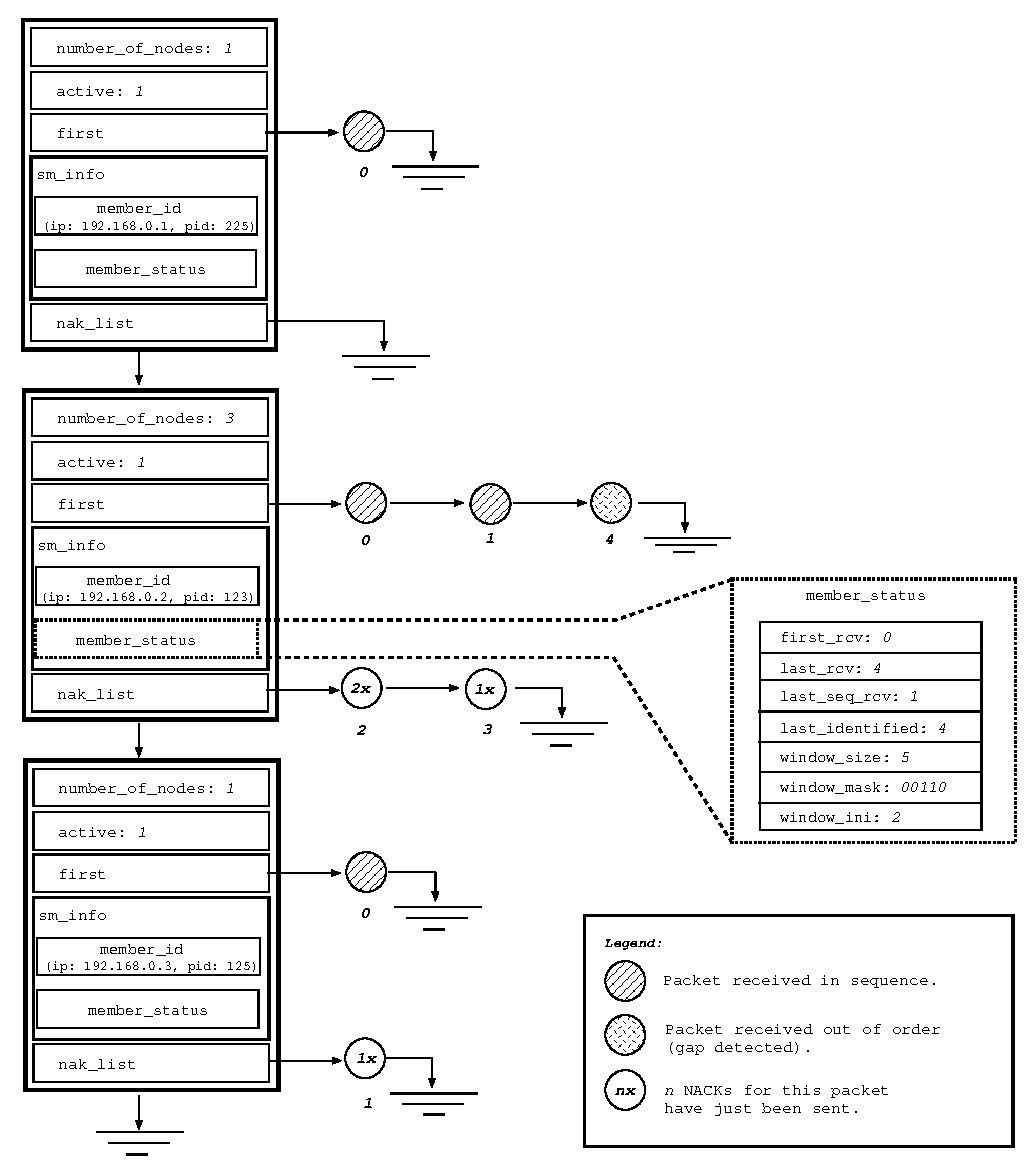
\includegraphics[%
  width=1.0\columnwidth]{cache.eps}\end{center}


\caption{\label{rml cache strucuture}RML Cache structure}
\end{figure}



\subsubsection{Loss Detection}

When a member of the multicast group receives a data packet, he checks
the packet sequence number and the sender identification. Then, the
member tries to match the sender identification with some \emph{member\_id}
in his cache. If he is successful in that matching, the sender is
already in the cache. Otherwise a node for the new member must be
inserted in the cache. After that, the member has to check whether
or not the received packet is in sequence. 

If the sequence number (sn) is in order, i.e., \texttt{sn=last\_seq\_rcv+1},
the packet is inserted in the cache and passed to the application.
If the sequence number is not in sequence, the member has found out
that packets were lost - a gap was detected. Detected the loss, it
is necessary to execute the procedures for recovering the lost packets.
The data packet received out of order is inserted and kept in the
cache. It will be released to the application after all lost data
have been recovered.

The recovery procedure consists of requesting retransmissions for
the lost data packets, in other words, to send NACK messages for the
multicast group. For instance, as it can be seen in figure \ref{rml cache strucuture},
if the losses of data packets 2 and 3 were detected, then the member
is supposed to send requests for retransmission of those data packets.
Any member of the multicast session that has the requested data is
able to retransmit it. In that way, the retransmission responsibility
is distributed.

The loss detection discussed before can fail when the lost packet
is the last packet transmitted by the sender. Suppose that a member
A has sent his last data packet with sn=10 and that member B has lost
that packet. Member B is unable to detect the loss until he receives
a new data packet from member A. But we have supposed that A will
not send new packets. In that situation, there must be another way
of detecting the loss. To solve that problem, members send a {}``
refresh message'' periodically indicating the sn of the last packet
sent. When a member receives the {}``refresh message'', he is able
to identify the lost packets and to start the recovering procedures.
In our example, member B would receive a {}``refresh message'' from
member A and then would be able to detect and recover the lost packet.


\subsubsection{Sending NACKs}

Suppose a scenario where a member of the multicast group sends a data
packet to the other members, and all the other members lose that packet.
Now, suppose that a NACK packet is sent by every member immediately
after the loss is detected. That action may cause an unnecessary traffic
in the network. That problem is called NACK implosion\cite{key-36}.
One solution is to wait for a random time T\emph{\footnotesize nack}
before sending a NACK message. As other members of the multicast group
might have lost the same data message, and considering that T\emph{\footnotesize nack}
is random, there will be a member who will choose a smaller timer
and send the NACK message before the others. If before T\emph{\footnotesize nack}
expires the member receives a NACK message or a retransmission of
the lost data, the transmission of the NACK message will be canceled.
So, if we choose an efficient way to determine T\emph{\footnotesize nack}
we will have a great probability of suppressing the sending of duplicated
NACK messages through the network.

Besides the implosion of NACKs, another problem that may happen related
to the sending of NACK messages is that the member may request more
data than he is able to handle. In fact, this two problems are similar
to the ones faced in the unicast case. The congestion control, used
in the TCP, is implemented in order to avoid network congestion. The
flow control, also used in the TCP, tries to get rid of the buffer
overflow in the client application. More information about TCP mechanisms
can be found in chapter 3 of \cite{key-3}. As described in the last
paragraph, the NACK suppression algorithm tries to solve a problem
analog to the one solved by the congestion control in the unicast
case. In that way, the congestion control and NACK suppression algorithm
attempt to avoid a network core congestion while the unicast and multicast
flow control attempt to prevent the overflow that may happen at the
network hosts (end systems) buffers. RML implements a simple flow
control: the amount of NACKs sent should not exceed the amount of
data that the member expecting this packets may process at once. 

%
\begin{figure}[hbpt]
\begin{center}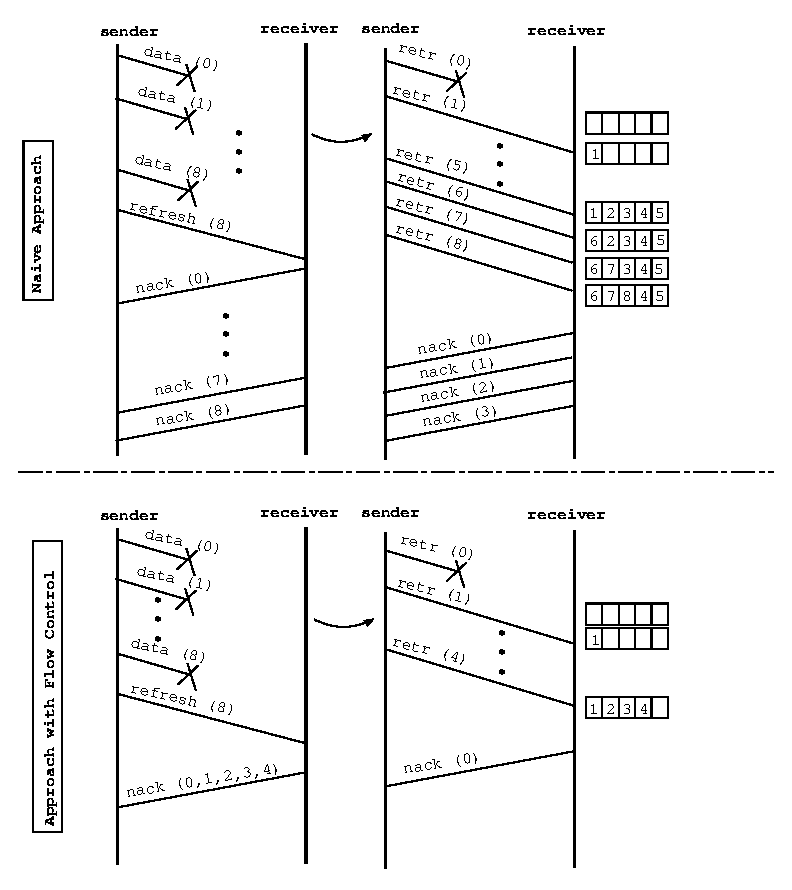
\includegraphics{flowcontrol.eps}\end{center}


\caption{\label{rml flow control}RML Flow Control}
\end{figure}


Two possible scenarios for flow control are illustrated in figure
\ref{rml flow control}. Suppose that packets with sn from 0 to 8
were transmitted by the sender. Those packets were lost by the receiver.
The receiver detects the loss when he receives a refresh message from
the sender. Then there are two ways of dealing with that loss. The
first approach, which we call \emph{Naive Approach}, is, in fact,
an approach with no flow control. The problem with this approach is
that the receiver will send a large amount of NACK messages and it
may happen that the amount of retransmission received in response
to those NACKs may be greater than the cache space available. Thus,
old data packets, that have not already been sent to the application,
will be replaced by new ones. In figure \ref{rml flow control} the
packet with sn 0 was lost. The receiver has a cache with five slots.
It may be seen that data packets from 1 to 5 were first stored in
the cache. Note that those packets were not sent to the application
because the packet with sn 0 is missed. Then, packets from 6 to 8
were received and replaced packets 1, 2 and 3. After that, the receiver
must send NACKs to recover packets from 0 to 3. We can see that it
is not useful to replace packets that have not already been sent to
the application.

In the second approach, which we call \emph{Flow Control Approach},
when a loss is detected the receiver only send NACKs for a certain
amount of packets, i.e., the amount he is able to handle. In addition,
the receiver requests those retransmissions in only one NACK message.
Note in figure \ref{rml flow control} that the first NACK sent requests
retransmissions for packets with sn 0 to 4 because there were five
free slots in the cache. The second NACK requests only the retransmission
of packet 0 because there was only one free slot in the cache at that
time. Using the Flow Control Approach two NACKs were sent, while in
the Naive Approach they were thirteen.

%
\begin{figure}[hbpt]
\begin{center}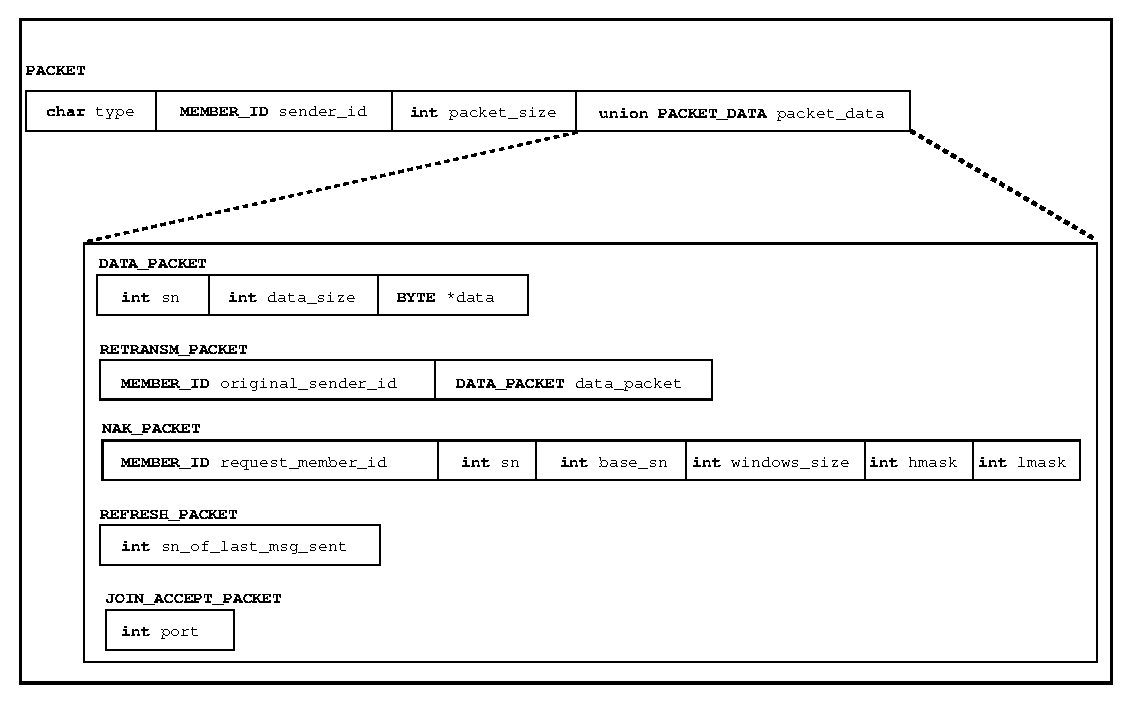
\includegraphics[%
  width=1.0\columnwidth]{packet_types.eps}\end{center}


\caption{\label{rml packet types}RML Packet Types}
\end{figure}


The RML uses the \emph{window\_mask}, \emph{window\_size} and \emph{window\_ini}
parameters to bound the NACK transmission. The \emph{window\_size}
has a value of 64, i.e., we can request at most 64 retransmissions
per NACK message. The \emph{window\_size} value was chosen just for
implementation purposes. With that value we can represent the \emph{window\_mask}
using only two integers in the NACK packets, as shown in figure \ref{rml nack mask}.
The \emph{window\_ini} points to the first position in the \emph{window\_mask}
array. The NACK packet is mounted using those parameters. In figure
\ref{rml packet types}, there is a description of the packet structures
used in RML. The NACK packet is composed by a set of fields, among
them we have :

\begin{itemize}
\item \textbf{base\_sn:} the value of the sn of the first NACK in the \emph{window\_mask}
\item \textbf{window\_size:} the value of \emph{window\_size} of the cache,
default is 64
\item \textbf{hmask:} an integer that represents the higher part of the
NACK mask
\item \textbf{lmask:} an integer that represents the lower part of the NACK
mask
\end{itemize}
%
\begin{figure}[hbpt]
\begin{center}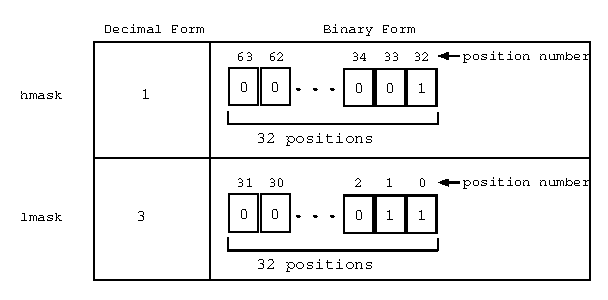
\includegraphics{nack_mask.eps}\end{center}


\caption{\label{rml nack mask}RML NACK mask}
\end{figure}


Suppose a NACK message from member M has arrived with \emph{base\_sn=5,
window\_size=64, hmask=1} and \emph{lmask=3.} To find out which retransmission
has been requested by member M we have to translate \emph{hmask} and
\emph{lmask} to their binary representation. This translation is shown
in figure \ref{rml nack mask}. The requests can be identified using
the position of the bits with value of 1 plus the \emph{base\_sn}.
In our scenario, the requests are for the packets with sn 5 (0+5),
6 (1+5) and 37 (32+5).

After sending a NACK message, the member waits for a retransmission
during a random period of time, called T\emph{\footnotesize wait}.
If the requested retransmission is not received after T\emph{\footnotesize wait}
units of time, a new NACK message is sent. The maximum number of NACKs
is limited by {\small the MAX\_NAK} parameter, which the user may
set in the rmcast.config file (see section 5.3 to learn about RML
configuration). If MAX\_NAK is reached, i.e., a data packet couldn't
be recovered - the application is then suspended. 


\subsubsection{Data Retransmission}

In the RML each member maintains in his cache the last N data packets
he has received from other members. Thus, any member of the multicast
group is able to answer to a request for retransmission of the last
N messages he has received from each other member. This mechanism
distributes the responsibility of retransmission among all the members
of the multicast session, but it may create a lot of traffic if every
member answers to a NACK message. As was explained in section 4.3.3,
we use random timers to avoid this traffic problem.

Suppose a member A receives a NACK message from member B regarding
a specific lost packet P from member C. If the packet P is stored
in A's cache, then member A schedules a random timer T\emph{\footnotesize ret}
to wait before sending a retransmission. There are two situations
that may occur before T\emph{\footnotesize ret} timed out:

\begin{enumerate}
\item a retransmission of the packet P is received: the A's retransmission
is aborted because another member has already answered the request.
\item a NACK message regarding the same packet P is received: the NACK message
is ignored because the retransmission is already scheduled.
\end{enumerate}
If T\emph{\footnotesize ret} expires and neither (1) nor (2) has occurred,
then the retransmission is sent.


\subsection{The Event List }

A common activity of the reliable multicast library (RML) is to schedule
an event to happen some time in the future. Almost every action that
is taken by the RML is not executed immediately when it is requested.
Instead, events are scheduled in order to perform the tasks. When
a loss of packets is detected, for example, an event is scheduled
to send a negative acknowledgment (NACK) after a certain period of
time. If, before the timeout, the member receives a retransmission
of the lost packet or if the member receives a NACK for the considered
packet, then the sending of the NACK is canceled. In the last case,
the sending of the NACK is suppressed because another member has just
sent the NACK. In order to reduce the network traffic, a member just
sends a message after waiting to see if this message was just sent
by another member. The key point here is to keep the work distributed
but avoiding redundancy.

The event list of the Reliable Multicast Protocol is an implementation
of a conventional delta list \cite{key-37}. The list is a chain of
event nodes. The event nodes are stored in increasing order of when
the event occurs. Each event node contains the information needed
to execute the event - the event type, described below, and some other
information, depending on the event type - as well as the time in
the future that the event should take place. The time stored in each
event is relative to the preceding event. For example, suppose there
are five events scheduled for 4, 6, 6, 13 and 17 time units in the
future. This would result in the event list illustrated in figure
\ref{rml simple event list}. Notice that the third event record contains
a 0 because it occurs 0 time units after the second event.

%
\begin{figure}[hbpt]
\begin{center}\includegraphics{simple_event_list.eps}\end{center}


\caption{\label{rml simple event list}RML Event List - a simple example}
\end{figure}


The first event node is the next one that will be executed. When an
event is inserted at the head of the list, an operating system alarm
signal is scheduled to fire after the time indicated at the header
node of the list. When the alarm fires, the event node is processed
and removed. All the subsequent events that have time of 0 are also
executed and removed. Then the alarm is restarted.

To schedule a new event, the event manager walks down the list and
inserts a record for the new event in the appropriate location, being
careful to adjust the relative time of both the new and the event
immediately following the new event. Deleting an event from the event
list is implemented in an analogous way.

The event nodes are divided into five types: 

\begin{itemize}
\item NAK\_SND\_WAIT- used to schedule a sending of a negative acknowledgment; 
\item RET\_RCV\_WAIT- used to wait for retransmissions; 
\item RET\_SND\_WAIT- created to schedule a sending of a retransmission; 
\item REF\_SND\_WAIT- used to schedule a refresh; 
\item LEV\_GRP\_WAIT- specifies the time between a user requests to go away
from the group and the actual moment when the user leaves the group.
\end{itemize}
Suppose there is one NAK\_SND\_WAIT event scheduled for 4 time units
in the future, in order to send a NACK to a packet initially sent
by member M1. Suppose also that there is one REF\_SND\_WAIT scheduled
for 6 time units in the future, and a RET\_SND\_WAIT for 17 time units
in the future. This retransmission refers to packet 4 of member M2.
This would result in the event list illustrated in figure \ref{rml detailed event list}.
Note that the NAK\_SND\_WAIT event node contains a pointer to the
cache entry of member M1. The cache entry of M1 will contain the information
about what packets from member M1 were lost. When the event NAK\_SND\_WAIT
fires, searching the cache we will find out which packets of member
M1 were lost, and then send a NACK message to request these packets.
On the other hand, the REF\_SND\_WAIT does not require any other information.
Finally, the RET\_SND\_WAIT schedules a retransmission, and to identify
the message to be retransmitted we need both the member id of the
message and its sequence number.

%
\begin{figure}[hbpt]
\begin{center}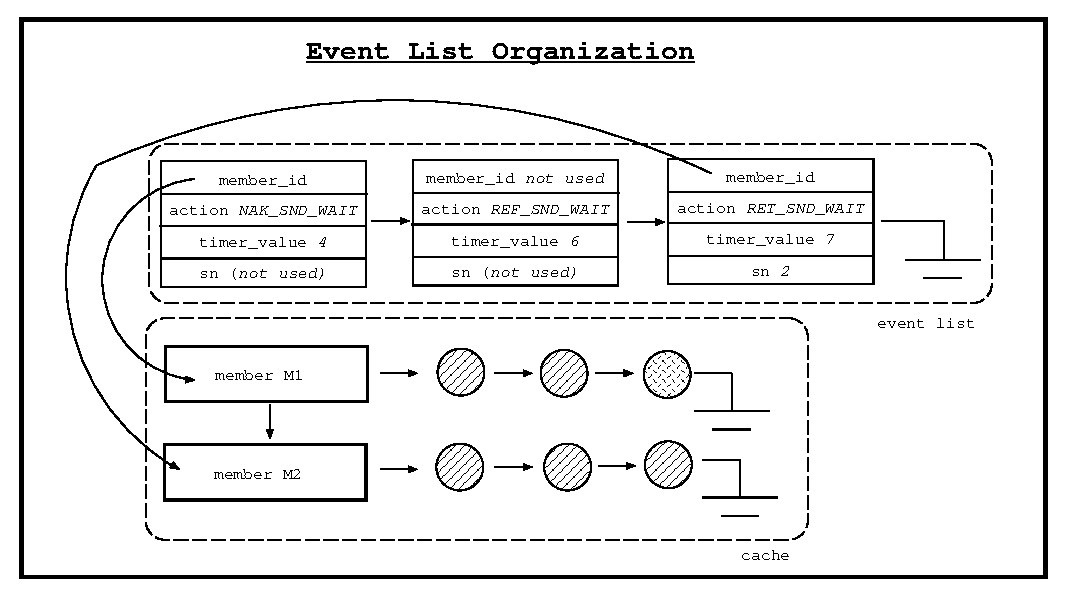
\includegraphics[%
  width=1.0\columnwidth]{eventlist.eps}\end{center}


\caption{\label{rml detailed event list}RML Event List - a more detailed
example}
\end{figure}


Figure \ref{rml event handlers} depicts how the different events
are handled.

%
\begin{figure}[hbpt]
\begin{center}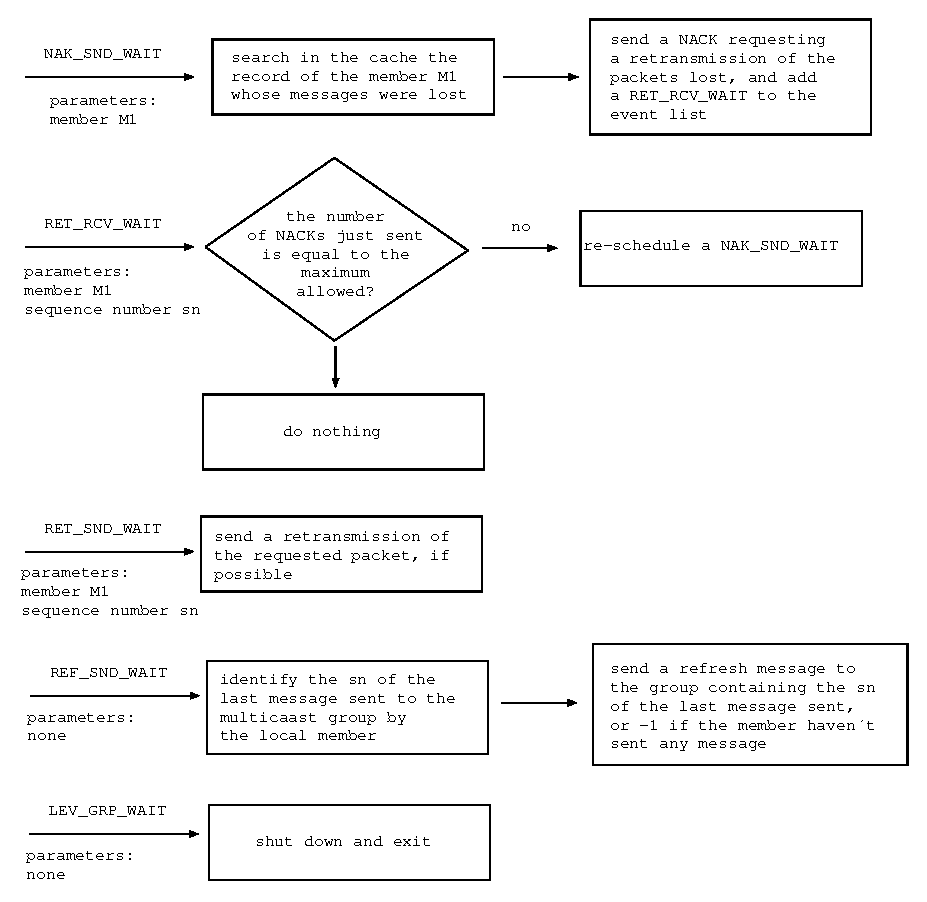
\includegraphics[%
  width=1.0\columnwidth]{fleventlist.eps}\end{center}


\caption{\label{rml event handlers}RML Event Handlers}
\end{figure}



\subsection{RML log generation}

The RML offers the option of log generation. The log file name is
configured through the LOG\_FILE option (see section 5.3 for further
information about RML parameters configuration). The file will be
created at the current directory and the host name and process ID
will be appended to the file name provided in the LOG\_FILE option.
Suppose LOG\_FILE=\emph{log} and the application that uses the RML
is called from the \emph{/tmp} directory at the \emph{machine01}.
Then, the log file name will be \emph{/tmp/log.machine01.137}, where
\emph{137} is the process ID of the application.

A log file sample is showed below:

\texttt{\scriptsize \hfill{}}~\\
\texttt{\scriptsize host: receiverhost}~\\
\texttt{\scriptsize ip: 192.168.1.2}~\\
\texttt{\scriptsize pid: 18348}~\\
\texttt{\scriptsize -{}-{}-{}-{}-{}-{}-{}-{}-{}-{}-{}-{}-{}-{}-{}-{}-{}-{}-{}-{}-{}-{}-{}-{}-{}-{}-{}-{}-{}-{}-{}-{}-{}-{}-{}-{}-{}-{}-{}-{}-{}-{}-{}-{}-{}-{}-{}-{}-{}-{}-{}-{}-{}-{}-{}-{}-{}-{}-{}-{}-{}-{}-{}-{}-{}-{}-{}-{}-{}-{}-{}-{}-{}-{}-{}-{}-{}-{}-{}-{}-{}-{}-{}-{}-{}-{}-{}-{}-{}-{}-{}-{}-{}-{}-{}-{}-{}-{}-{}-{}-{}-{}-{}-{}-{}-{}-{}-{}-{}-{}-{}-{}-{}-{}-}~\\
\texttt{\scriptsize time snd/rcv/loss type sender\_ip~ sender\_pid
requested\_ip~ requested\_pid sn~ {[}\{base\_sn\} \{win\_size\}
\{hmask\} \{lmask\}{]}}~\\
\texttt{\scriptsize -{}-{}-{}-{}-{}-{}-{}-{}-{}-{}-{}-{}-{}-{}-{}-{}-{}-{}-{}-{}-{}-{}-{}-{}-{}-{}-{}-{}-{}-{}-{}-{}-{}-{}-{}-{}-{}-{}-{}-{}-{}-{}-{}-{}-{}-{}-{}-{}-{}-{}-{}-{}-{}-{}-{}-{}-{}-{}-{}-{}-{}-{}-{}-{}-{}-{}-{}-{}-{}-{}-{}-{}-{}-{}-{}-{}-{}-{}-{}-{}-{}-{}-{}-{}-{}-{}-{}-{}-{}-{}-{}-{}-{}-{}-{}-{}-{}-{}-{}-{}-{}-{}-{}-{}-{}-{}-{}-{}-{}-{}-{}-{}-{}-{}-}~\\
\texttt{\scriptsize 51800783466~~ L~~ RF~~ 192.168.1.1~ 13893~~~~~~~~~~~~~~~~~~~~~~~~~~~~~~~~
-1}~\\
\texttt{\scriptsize 51808642569~~ L~~ DT~~ 192.168.1.1~ 13893~~~~~~~~~~~~~~~~~~~~~~~~~~~~~~~~~
0}~\\
\texttt{\scriptsize 51810314729~~ S~~ RF~~ 192.168.1.2~ 18348~~~~~~~~~~~~~~~~~~~~~~~~~~~~~~~~
-1}~\\
\texttt{\scriptsize 51829942926~~ R~~ DT~~ 192.168.1.1~ 13893~~~~~~~~~~~~~~~~~~~~~~~~~~~~~~~~
48}~\\
\texttt{\scriptsize 51829947209~~ S~~ NK~~ 192.168.1.2~ 18348~
192.168.1.1~~~~~~~~~ 13893~~~~~~~~~~ -1~~~~~~~~~
64~~~~ 29280~ 235372671}~\\
{\scriptsize \par}

The header of the log file is composed by the host name, ip address
and process ID. Then a short description of the log structure is presented.
After that, each line describe a packet that was received or sent
by the member. The fields are:

\begin{itemize}
\item \textbf{time:} indicates the time when the packet was received or
sent
\item \textbf{snd/rcv/loss:} indicates if the packet was sent (S), received
(R) or received but lost because of loss simulation (L).
\item \textbf{type:} indicates the packet type, i.e., NACK(NK), data(DT),
retransmission(RT), refresh(RF), join accept(JA), join request(JR),
leave group(LG) and unknown(UN).
\item \textbf{sender\_ip:} indicates the IP address of the sender
\item \textbf{sender\_pid:} indicates the process ID of the sender
\item \textbf{requested\_ip:} this field appears when a NACK or a retransmission
packet is received. If the NACK is requesting the retransmission from
packets sent by member C, this field indicates C's IP address.
\item \textbf{requested\_pid:} this field only appears when a NACK or a
retransmission packet is received. If the NACK is requesting the retransmission
from packets sent by member C, this field indicates C's process ID.
\item \textbf{sn:} this field has different meanings depending on the packet
type. When the packet is data or retransmission, this field indicates
the sequence number of the packet. When the packet is a refresh message,
this field indicates the sequence number of the last data packet sent
by the member identified by sender\_ip and sender\_pid. This field
does not appear for the remaining packet types.
\item \textbf{base sn:} indicates the value of the sequence number of the
first retransmission requested in the NACK packet.
\item \textbf{win size:} indicates the window size of the NACK packet
\item \textbf{hmask:} an integer that represents the higher part of the
NACK mask
\item \textbf{lmask:} an integer that represents the lower part of the NACK
mask
\end{itemize}
There is a simple shell script, called rmcastplot.bash, that can be
used to generate statistics and plots from the RML log files. If you
run rmcastplot.bash with no arguments it will show a short help:


\paragraph{\texttt{\textmd{\footnotesize -{}-{}-{}-{}-{}-{}-{}-{}-{}-{}-{}-{}-{}-{}-{}-{}-{}-{}-{}-{}-{}-{}-{}-{}-{}-{}-{}-{}-{}-{}-{}-{}-{}-{}-{}-{}-{}-{}-{}-{}-{}-{}-{}-{}-{}-{}-{}-{}-{}-{}-{}-{}-{}-{}-{}-{}-{}-{}-{}-{}-{}-{}-{}-{}-{}-{}-{}-{}-{}-{}-{}-{}-{}-{}-{}-{}-{}-{}-{}-{}-{}-{}-{}-{}-{}-{}-{}-{}-{}-{}-{}-{}-{}-{}-{}-{}-{}-{}-{}-{}-}}~\protect \\
\texttt{\textmd{\footnotesize Usage:}}~\protect \\
\texttt{\textmd{\footnotesize rmcastplot.bash <max\_num\_pack\_sent>
<xyrange> <member1.log> <member2.log> {[}awk\_script\_dir{]} {[}tgif|png{]}}}~\protect \\
\texttt{\textmd{\footnotesize ~}}~\protect \\
\texttt{\textmd{\footnotesize max\_num\_pack\_sent: maximum number
of sent packets}}~\protect \\
\texttt{\textmd{\footnotesize xyrange: {[}XMIN:XMAX{]}{[}YMIN:YMAX{]}
gnuplot style}}~\protect \\
\texttt{\textmd{\footnotesize member1.log: full path to member log}}~\protect \\
\texttt{\textmd{\footnotesize member2\_log: full path to member log}}~\protect \\
\texttt{\textmd{\footnotesize awk\_script\_dir: optional parameter. Full
path to directory where rmlog.awk script is found}}~\protect \\
\texttt{\textmd{\footnotesize tgif or png: optional parameter. Changes
gnuplot output to generate Tgif files or PNG files}}~\protect \\
\texttt{\textmd{\footnotesize -{}-{}-{}-{}-{}-{}-{}-{}-{}-{}-{}-{}-{}-{}-{}-{}-{}-{}-{}-{}-{}-{}-{}-{}-{}-{}-{}-{}-{}-{}-{}-{}-{}-{}-{}-{}-{}-{}-{}-{}-{}-{}-{}-{}-{}-{}-{}-{}-{}-{}-{}-{}-{}-{}-{}-{}-{}-{}-{}-{}-{}-{}-{}-{}-{}-{}-{}-{}-{}-{}-{}-{}-{}-{}-{}-{}-{}-{}-{}-{}-{}-{}-{}-{}-{}-{}-{}-{}-{}-{}-{}-{}-{}-{}-{}-{}-{}-{}-{}-{}-}}}


\paragraph{\texttt{\textmd{\footnotesize ~}}}

Suppose there are two members using an RML based application. They
generate two log files: log.senderhost.13893 and log.receiverhost.18348.
For instance, rmcastplot.bash script can be executed with the following
line command:

\begin{center}\texttt{\footnotesize \hfill{}}~\\
\texttt{\footnotesize rmcastplot.bash 100 {[}0:15{]}{[}0:5{]} log.senderhost.13893
log.receiverhost.18348}~\\
\texttt{\footnotesize \hfill{}}\end{center}{\footnotesize \par}

The script outputs some statistics at the standard input:

\texttt{\footnotesize \hfill{}}{\footnotesize \par}

\texttt{\footnotesize -{}-{}-{}-{}-{}-{}-{}-{}-{}-{}-{}-{}-{}-{}-{}-{}-{}-{}-{}-{}-{}-{}-{}-{}-{}-{}-{}-{}-{}-{}-{}-{}-{}-{}-{}-{}-{}-{}-{}-{}-{}-{}-{}-{}-{}-{}-{}-{}-{}-}{\footnotesize \par}

\texttt{\footnotesize Member 1 Name:~ senderhost}{\footnotesize \par}

\texttt{\footnotesize Member 1 IP:~ 192.168.1.1}{\footnotesize \par}

\texttt{\footnotesize Member 1 PID: 13893}{\footnotesize \par}

\texttt{\footnotesize Member 2 Name:~ receiverhost}{\footnotesize \par}

\texttt{\footnotesize Member 2 IP:~ 192.168.1.2}{\footnotesize \par}

\texttt{\footnotesize Member 2 PID: 18348}{\footnotesize \par}

\texttt{\footnotesize -{}-{}-{}-{}-{}-{}-{}-{}-{}-{}-{}-{}-{}-{}-{}-{}-{}-{}-{}-{}-{}-{}-{}-{}-{}-{}-{}-{}-{}-{}-{}-{}-{}-{}-{}-{}-{}-{}-{}-{}-{}-{}-{}-{}-{}-{}-{}-{}-{}-}{\footnotesize \par}

\texttt{\footnotesize ~ Data related to}{\footnotesize \par}

\texttt{\footnotesize ~ log.senderhost.13893 -> 192.168.1.2:18348}{\footnotesize \par}

\texttt{\footnotesize -{}-{}-{}-{}-{}-{}-{}-{}-{}-{}-{}-{}-{}-{}-{}-{}-{}-{}-{}-{}-{}-{}-{}-{}-{}-{}-{}-{}-{}-{}-{}-{}-{}-{}-{}-{}-{}-{}-{}-{}-{}-{}-{}-{}-{}-{}-{}-{}-{}-}{\footnotesize \par}

\texttt{\footnotesize Data sent:~~~ 101}{\footnotesize \par}

\texttt{\footnotesize Data received from 192.168.1.2:18348~~ 1}{\footnotesize \par}

\texttt{\footnotesize NACKs sent:~~~~ 0}{\footnotesize \par}

\texttt{\footnotesize NACKs received from 192.168.1.2:18348~~~
5}{\footnotesize \par}

\texttt{\footnotesize Refresh sent:~ 9}{\footnotesize \par}

\texttt{\footnotesize Refresh received from 192.168.1.2:18348 16}{\footnotesize \par}

\texttt{\footnotesize Retrans sent:~ 51}{\footnotesize \par}

\texttt{\footnotesize Retrans received from 192.168.1.2:18348 0}{\footnotesize \par}

\texttt{\footnotesize Total simulated loss:~~ 0}{\footnotesize \par}

\texttt{\footnotesize Data loss with simulation from 192.168.1.2:18348~~~
0}{\footnotesize \par}

\texttt{\footnotesize NACKs lost by simulation from 192.168.1.2:18348~~~
0}{\footnotesize \par}

\texttt{\footnotesize Refresh lost by simulation from 192.168.1.2:18348~~~
0}{\footnotesize \par}

\texttt{\footnotesize Retrans lost by simulation from 192.168.1.2:18348~~~
0}{\footnotesize \par}

\texttt{\footnotesize Packets identified:~ 517}{\footnotesize \par}

\texttt{\footnotesize -{}-{}-{}-{}-{}-{}-{}-{}-{}-{}-{}-{}-{}-{}-{}-{}-{}-{}-{}-{}-{}-{}-{}-{}-{}-{}-{}-{}-{}-{}-{}-{}-{}-{}-{}-{}-{}-{}-{}-{}-{}-{}-{}-{}-{}-{}-{}-{}-{}-}{\footnotesize \par}

\texttt{\footnotesize ~}{\footnotesize \par}

\texttt{\footnotesize -{}-{}-{}-{}-{}-{}-{}-{}-{}-{}-{}-{}-{}-{}-{}-{}-{}-{}-{}-{}-{}-{}-{}-{}-{}-{}-{}-{}-{}-{}-{}-{}-{}-{}-{}-{}-{}-{}-{}-{}-{}-{}-{}-{}-{}-{}-{}-{}-{}-}{\footnotesize \par}

\texttt{\footnotesize ~ Data related to}{\footnotesize \par}

\texttt{\footnotesize ~ log.receiverhost.18348 -> 192.168.1.1:13893}{\footnotesize \par}

\texttt{\footnotesize -{}-{}-{}-{}-{}-{}-{}-{}-{}-{}-{}-{}-{}-{}-{}-{}-{}-{}-{}-{}-{}-{}-{}-{}-{}-{}-{}-{}-{}-{}-{}-{}-{}-{}-{}-{}-{}-{}-{}-{}-{}-{}-{}-{}-{}-{}-{}-{}-{}-}{\footnotesize \par}

\texttt{\footnotesize Data sent:~~~ 1}{\footnotesize \par}

\texttt{\footnotesize Data received from 192.168.1.1:13893~~ 65}{\footnotesize \par}

\texttt{\footnotesize NACKs sent:~~~~ 5}{\footnotesize \par}

\texttt{\footnotesize NACKs received from 192.168.1.1:13893~~~
0}{\footnotesize \par}

\texttt{\footnotesize Refresh sent:~ 7}{\footnotesize \par}

\texttt{\footnotesize Refresh received from 192.168.1.1:13893 11}{\footnotesize \par}

\texttt{\footnotesize Retrans sent:~ 0}{\footnotesize \par}

\texttt{\footnotesize Retrans received from 192.168.1.1:13893 36}{\footnotesize \par}

\texttt{\footnotesize Total simulated loss:~~ 54}{\footnotesize \par}

\texttt{\footnotesize Data loss with simulation from 192.168.1.1:13893~~~
36}{\footnotesize \par}

\texttt{\footnotesize NACKs lost by simulation from 192.168.1.1:13893~~~
0}{\footnotesize \par}

\texttt{\footnotesize Refresh lost by simulation from 192.168.1.1:13893~~~
3}{\footnotesize \par}

\texttt{\footnotesize Retrans lost by simulation from 192.168.1.1:13893~~~
15}{\footnotesize \par}

\texttt{\footnotesize Packets identified:~ 453 }{\footnotesize \par}

\texttt{\footnotesize -{}-{}-{}-{}-{}-{}-{}-{}-{}-{}-{}-{}-{}-{}-{}-{}-{}-{}-{}-{}-{}-{}-{}-{}-{}-{}-{}-{}-{}-{}-{}-{}-{}-{}-{}-{}-{}-{}-{}-{}-{}-{}-{}-{}-{}-{}-{}-{}-{}-}{\footnotesize \par}

\hfill{}

Besides those statistics, if you have gnuplot\cite{key-38} installed
in your system, some plots will be generated. One of those plots is
showed in figure \ref{log plot}.

%
\begin{figure}[hbpt]
\begin{center}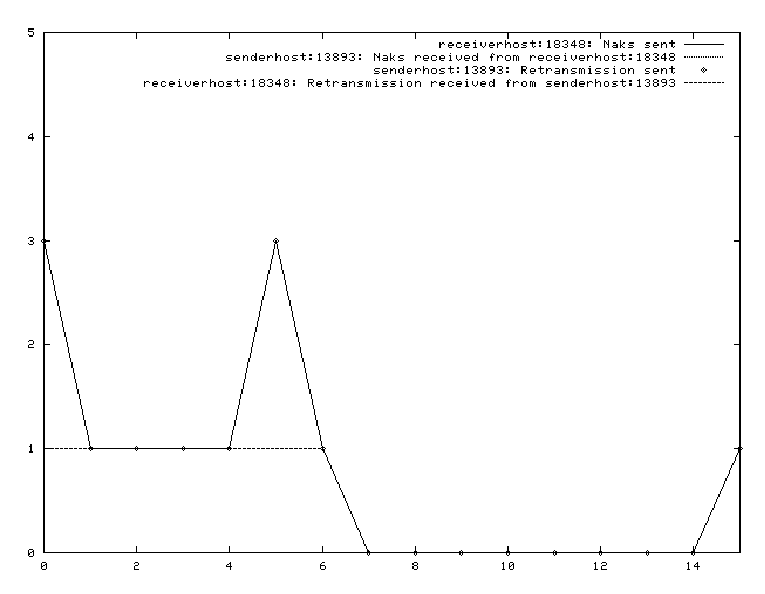
\includegraphics{log_plot.eps}\end{center}


\caption{\label{log plot}Log plotted with the rmcastplot.bash script}
\end{figure}



\subsection{Summary}

Figure \ref{rml actions on receiving packets} summarizes the RML
behavior on receiving each packet type.

%
\begin{figure}[hbpt]
\begin{center}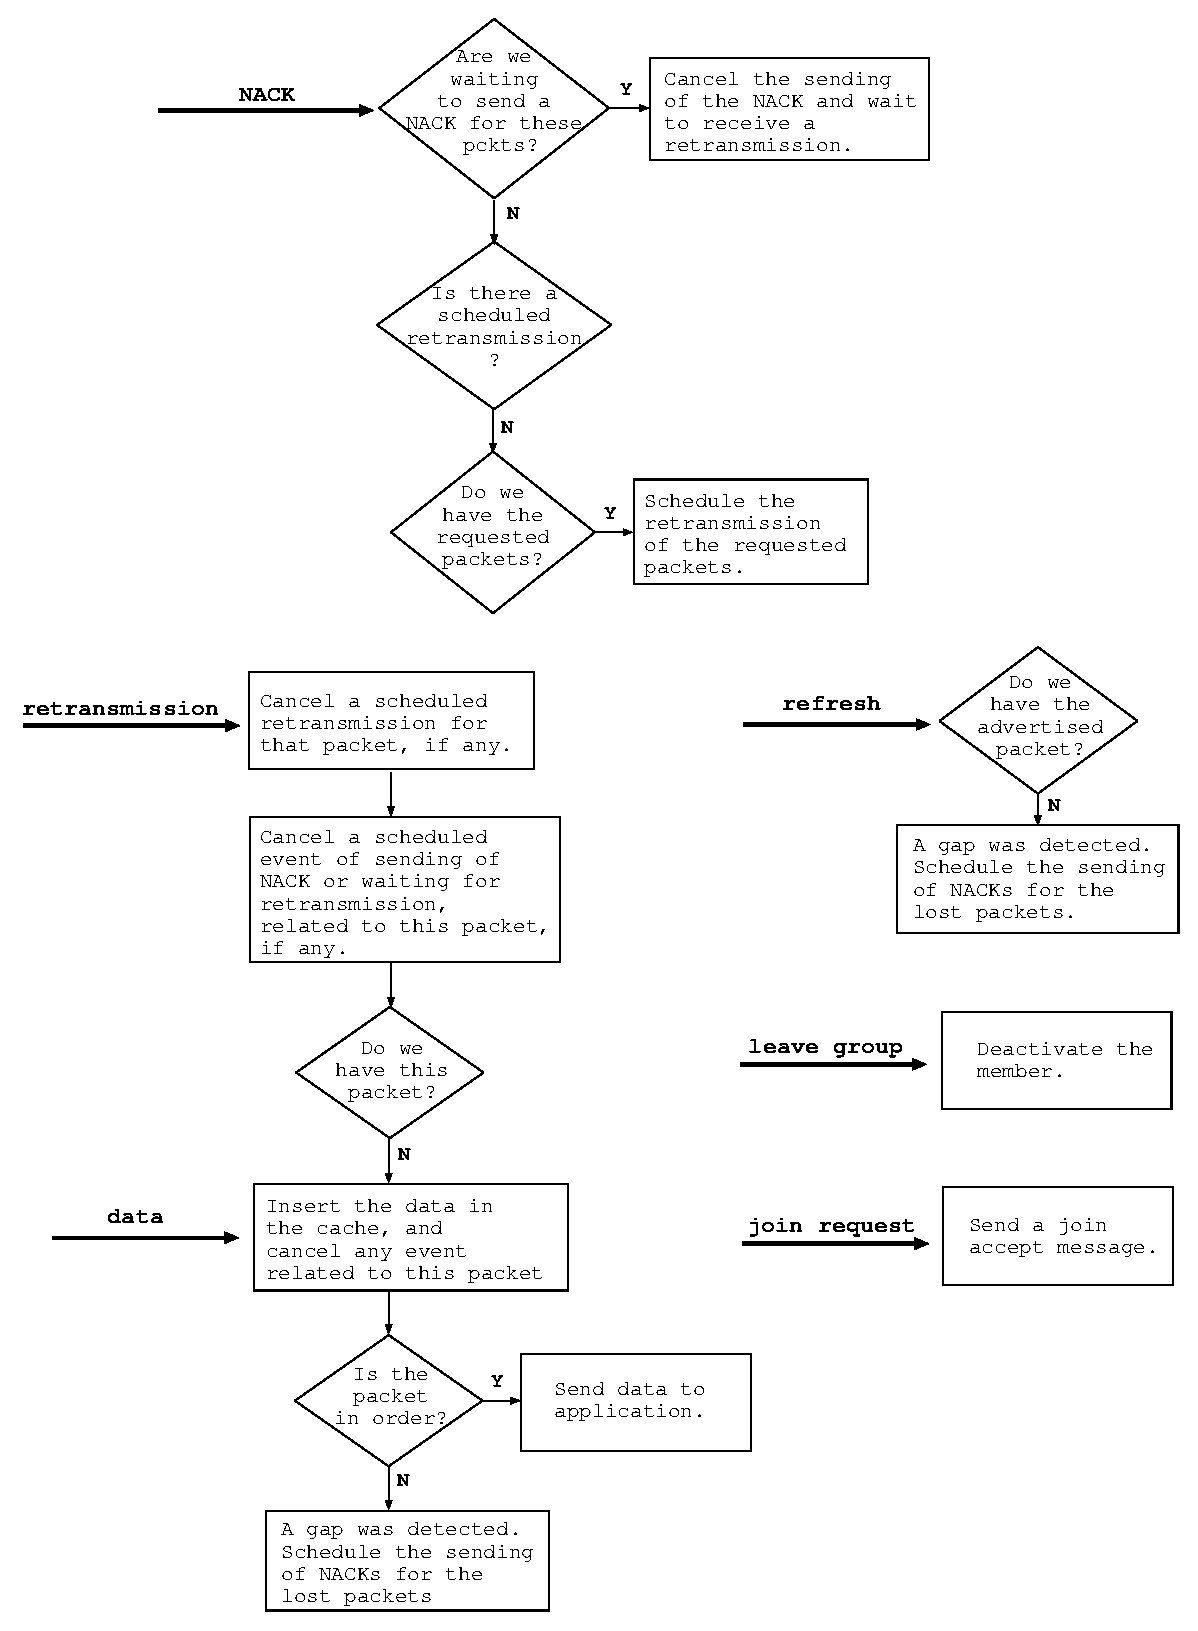
\includegraphics[%
  width=1.0\textwidth,
  height=1.0\textwidth]{actions_on_receiving_packets.eps}\end{center}


\caption{\label{rml actions on receiving packets}Actions taken on receiving
each packet type}
\end{figure}



\section{A simple example: the chat program }

In this section we will describe a simple chat application that uses
the RML. We hope that this simple example may be used to show how
to develop an application based on our RML.


\subsection{Minimal requirements to create an Reliable Multicast based application}

The development of a Reliable Multicast application has some requirements
as follow:

\begin{itemize}
\item A multicast enabled environment (see section 2 to learn about that);
\item The Reliable Multicast Library - the librmcast.a file;
\item The Reliable Multicast Header - the rmcast.h file;
\item C language develop environment - gcc, make, c libraries etc.
\end{itemize}

\subsection{Getting and installing the Reliable Multicast Library}

To get the Reliable Multicast Library do the following:

\begin{enumerate}
\item Download the RML source code from our project page at \emph{}\\
\emph{http://www.land.ufrj.br/tools/rmcast}
\item Gunzip and untar the package. After that the RelMulticast directory
will be created.
\item Change to RelMulticast directory.
\item Type make and see if the \textbf{librmcast.a} is compiled without
errors. This may be flawless for most users.
\end{enumerate}
To compile an application with librmcast.a you should use the following
options with gcc:

\begin{quote}
-I<rmcast.h\_directory> -L<librmcast.a\_directory> -lrmcast
\end{quote}
For instance, we have an application called rmchat in the examples/rmchat
directory, to compile that application we should issue the command:

\begin{quote}
gcc rmchat.c -I../.. -L../.. -lpthread -lm -lrmcast -o rmchat
\end{quote}
Inside the RelMulticast directory you will find some useful files
such as README, INSTALL etc. Those files contain the most updated
instructions to compile the RML, please take a look at them.


\subsection{The Reliable Multicast Library configuration}

There are two ways for an application to customize the Reliable Multicast
Library options:

\begin{enumerate}
\item Calling the \textbf{RM\_setOption(int OPTION\_ID, void {*}OPTION\_VALUE)}
function, where: \\
\\
OPTION\_ID: indicates what option you want to set. You can found the
option list in the rmcast.h header file. \\
OPTION\_VALUE: the value you want to set the option to \\
\\
\textbf{Example:} \\
\texttt{... }~\\
\texttt{/{*} Setting REFRESH\_TIMER {*}/ }~\\
\texttt{int refresh\_timer=10; }~\\
\texttt{}~\\
\texttt{RM\_setOption(REFRESH\_TIMER,(void {*}) refresh\_timer); }~\\
\texttt{... }
\item Calling \textbf{RM\_readConfigFile(char {*}filename)}. This function
will tell the Reliable Multicast Library to read the user's options
from \textbf{filename}. \\
\\
\textbf{Example:} \\
\\
\texttt{...}~\\
\texttt{/{*} Read the config file from /etc/rmcast.config {*}/ }~\\
\texttt{char config\_file{[}50{]}; }~\\
\texttt{}~\\
\texttt{strcpy(config\_file,\char`\"{}/etc/rmcast.config\char`\"{});
}~\\
\texttt{}~\\
\texttt{RM\_readConfigFile(config\_file); }~\\
\texttt{...} \\

\end{enumerate}
NOTE: There is a constant, RM\_USE\_CURRENT\_CONFIG, that can replace
functions parameters. In those situations, the RM\_USE\_CURRENT\_CONFIG
will indicate that the current values (which may have been set either
by calling RM\_setOption or RM\_readConfigFile) must be used. For
instance, when we call the RM\_joinGroup() function we are supposed
to pass as parameters the IP Multicast address and port number. If
we have already read those options from rmcast.config file, just replace
the parameters with the RM\_USE\_CURRENT\_CONFIG constant.\\


The rmcast.config file contain some options that can be customized
by the users. A rmcast.config file example follows (lines beginning
with a \"{ }\#\"{ } are comments):

\begin{quote}
\texttt{\footnotesize \#Reliable Multicast Library configuration file}{\footnotesize \par}

\texttt{\footnotesize \#Reliable Multicast Library version }~\\
\texttt{\footnotesize RM\_VERSION=1.0}{\footnotesize \par}

\texttt{\footnotesize \#Transmission mode: 0 multicast (default),
1 unicast }~\\
\texttt{\footnotesize TRANSMISSION\_MODE=0}{\footnotesize \par}

\texttt{\footnotesize \#Multicast or Unicast IP address to send data
(destination IP) }~\\
\texttt{\footnotesize DEST\_IP=225.1.2.3}{\footnotesize \par}

\texttt{\footnotesize \#Multicast or Unicast port to send data (destination
port) }~\\
\texttt{\footnotesize DEST\_PORT=5000}{\footnotesize \par}

\texttt{\footnotesize \#Time to live for the packets setting (1 indicates
local network) }~\\
\texttt{\footnotesize TTL=1}{\footnotesize \par}

\texttt{\footnotesize \#Inter-packet sleep timer - timer between transmissions
of packets }~\\
\texttt{\footnotesize \#( in microseconds) }~\\
\texttt{\footnotesize MICROSLEEP=10}{\footnotesize \par}

\texttt{\footnotesize \#Log file path - NULL disable logging (default)
}~\\
\texttt{\footnotesize LOG\_FILE=NULL}{\footnotesize \par}

\texttt{\footnotesize \#Random Timers Distribution: 0 uniform 1 exponential
}~\\
\texttt{\footnotesize TIMER\_DISTRIBUTION=0}{\footnotesize \par}

\texttt{\footnotesize \#Lower bound for timer generation (in milliseconds)
}~\\
\texttt{\footnotesize TIMER\_LOWER=200}{\footnotesize \par}

\texttt{\footnotesize \#Upper bound for timer generation (in milliseconds)
}~\\
\texttt{\footnotesize TIMER\_UPPER=1000}{\footnotesize \par}

\texttt{\footnotesize \#Max number of naks that can be sent for each
packet. 100 (default) }~\\
\texttt{\footnotesize MAX\_NAK=100}{\footnotesize \par}

\texttt{\footnotesize \# We will be able to retransmit the last MAX\_MEMBER\_CACHE\_SIZE
}~\\
\texttt{\footnotesize \# packets from each member of the multicast
group, i.e., we will store the}~\\
\texttt{\footnotesize \# last MAX\_MEMBER\_CACHE\_SIZE PACKETS from
each member}~\\
\texttt{\footnotesize \# of the multicast group in the cache. 4000
(default) }~\\
\texttt{\footnotesize \# }~\\
\texttt{\footnotesize \# WARNING: if you set MAX\_MEMBER\_CACHE\_SIZE
to low values }~\\
\texttt{\footnotesize \# the protocol may fail!! }~\\
\texttt{\footnotesize \# }~\\
\texttt{\footnotesize MAX\_MEMBER\_CACHE\_SIZE=4000 }{\footnotesize \par}

\texttt{\footnotesize \#Enable support for new users 1 enabled (default),
0 disabled }~\\
\texttt{\footnotesize NEW\_USER\_SUPPORT=0}{\footnotesize \par}

\texttt{\footnotesize \#Show transmission statistics: 0 disabled (default)
1 enabled }~\\
\texttt{\footnotesize STATISTICS=0}{\footnotesize \par}

\texttt{\footnotesize \#Time between sending of refresh messages (seconds)
}~\\
\texttt{\footnotesize REFRESH\_TIMER=10}{\footnotesize \par}

\texttt{\footnotesize \#Loss simulation: 0 disabled (default) any
float number > 0 enabled}{\footnotesize \par}

\texttt{\footnotesize \# A note about loss simulation: }~\\
\texttt{\footnotesize \# When loss simulation is enabled (LOSS\_PROB
> 0) we always loose }~\\
\texttt{\footnotesize \# the first 10 received packets, and the first
received data packet - }~\\
\texttt{\footnotesize \# that is, the first burst of received packets. }~\\
\texttt{\footnotesize \# After that, packets are lost according to
LOSS\_PROB. }~\\
\texttt{\footnotesize \# Example: LOSS\_PROB=30 }~\\
\texttt{\footnotesize \# The first 10 received packets will be lost. }~\\
\texttt{\footnotesize \# Then, 30\% of the packets will be lost }~\\
\texttt{\footnotesize LOSS\_PROB=0}{\footnotesize \par}

\texttt{\footnotesize \# Time to wait, in microseconds, before leaving
the multicast group. }~\\
\texttt{\footnotesize LEAVE\_GROUP\_WAIT\_TIME = 5000000}{\footnotesize \par}

\texttt{\footnotesize \# Size of the buffer of the receiver host }~\\
\texttt{\footnotesize \# (maximum size of a message that may be processed
by }~\\
\texttt{\footnotesize \# the receiver host).}~\\
\texttt{\footnotesize RCV\_BUFFER\_SIZE = 10000}{\footnotesize \par}
\end{quote}
To retrieve the current value of an option from the RML you must call
the \textbf{RM\_getOption(int OPTION,void {*}OPTION\_VALUE)} function\textbf{.}


\subsection{The Reliable Multicast Chat (rmchat) application}

This is a simple chat application and was written just for testing
the RML. The fully commented source code can be found in the examples/rmchat
directory. You can compile the program by typing \texttt{\textcolor{black}{make}}
in that directory. 


\subsubsection{The program}

Every user that initiates the program is prompted for a username -
this username will be the users identity in the group. After that
they will receive all the messages from every user already connected
to the chat group (if any). You can also type messages in the prompt
and send them to the group by pressing the return key. Note that there
is no need for a chat server because we are using multicast. Users
must know the IP address and port to join the chat group. You can
set this address and port through the rmcast.config file as we have
seen in the previous section. 

We have implemented only two simple commands in the rmchat:

\begin{enumerate}
\item \textbf{send -} by typing \texttt{\textcolor{black}{send}} on the
prompt you will be asked for the number of packets to send to the
group. This command was implemented to perform simple tests with the
application.
\item \textbf{exit} - this command is used to terminate the application.
\end{enumerate}

\subsubsection{Source code comments}

This section is supposed to be read along with the source code of
rmchat, available at examples/rmchat/rmchat.c.

The very first thing we have to do when we are writing an application
is to include the \textbf{rmcast.h} header file. Next we define BUFFSIZE
- the maximum message size. We also declare an integer global variable
to identify the socket we will use to send and receive data. 

The following step is to read the configuration file, calling the
\textbf{RM\_readConfigFile} function. Then, we have to initialize
the RML calling the \textbf{RM\_initialize} function. After that we
join the multicast group calling the \textbf{RM\_joinGroup} function.
At this point we are using the RM\_USE\_CURRENT\_CONFIG as discussed
in section 4.3. The \textbf{RM\_joinGroup} function returns the socket
identifier that we will need to send and receive data from the network.

Interactive network applications are supposed to simultaneously receive
and send data through the network. To implement that feature we usually
create separated threads to deal with those tasks. In the rmchat we
have created, calling the pthread\_create function, the \emph{}\textbf{Receive
thread} to receive packets from the network, while the main thread
will get the user messages and will send them to the multicast group.

You can easily see in the Receive thread code that there is a loop
where we just call \textbf{RM\_recv} function to retrieve data from
the network. The data received is then showed on the screen.

In the main program we are reading the messages typed by the user
and checking whether they are a command or a simple message. If it
is a simple message, we just call the \textbf{RM\_sendto} function
to send the data to the multicast group. Otherwise, if the \textbf{exit}
command is issued, we break the loop and prepare to terminate the
application. We use the \textbf{RM\_getOption} to retrieve the current
IP address and port from the RML just to report it to the user. In
addition we cancel the Receive thread using the pthread\_cancel()
function.

Finally we call the \textbf{RM\_leaveGroup} function to finish the
RML and our program. This function is \noun{very important} because
it cleans up the system resources that we were using such as the message
queue. See section 7.3 for further information on message queues.
Again, we recommend that you take a look at the source code to better
understand the application.


\subsection{RML functions quick reference}

In this section will go through the user functions available in the
Reliable Multicast Library.

\begin{itemize}
\item \textbf{RM\_readConfigFile(char {*}filename)} - read the configuration
file identified by \emph{filename}. See section 4.3 for the config
file format and options.
\item \textbf{RM\_setOption(int opt, void {*}optvalue)} - set the option
identified by \emph{opt} with the value in \emph{optvalue}. You can
use setOption to set the RML instead of reading the config file.
\item \textbf{RM\_getOption(int opt, void {*}optvalue)} - returns the current
value \emph{optvalue} of the option identified by \emph{opt}.
\item \textbf{RM\_initialize(void *callbackterm( void ))} - initializes the RML
structures and defines the callback function that will be used when finishing
the application
\item \textbf{RM\_getCurStatus(char {*}group, int port, CurStatus {*}c)}
- get the current status from a member of the multicast group.
\item \textbf{RM\_sendCurStatus(int connfd, char {*}buff, int buffsize)}
- send the current status to a new member of the multicast group.
\item \textbf{RM\_joinGroup(char {*}group, int port)} - join the multicast
group identified by the IP address in \emph{group} and the port in
\emph{port}. Returns the socket identifier that will be used in the
RM\_sendto and RM\_recv functions.
\item \textbf{RM\_sendto(int socket, void {*}buffer, int buffsize)} - sends
up to \emph{buffsize} bytes of data from \emph{buffer} using the socket
identifier \emph{socket}. Returns 1 on success and 0 if an error occurs.
\item \textbf{RM\_recv(int socket, void {*}buffer, int buffsize)} - receives
up to \emph{buffsize} bytes of data, and stores them into \emph{buffer}
using the socket identifier \emph{socket}. Returns the number of bytes
received on success and -1 when an error occurs.
\item \textbf{RM\_leaveGroup(int sock,char {*} group)} - sends a message
indicating that we are leaving the multicast group identified by \emph{group},
cleans all the system resources being used and closes the socket identified
by \emph{socket}. You must call this function before terminating the
application. Returns 1 on success and 0 on failure.
\end{itemize}

\section{A more advanced application: the Tangram II Whiteboard}


\subsection{About Tangram II Whiteboard (TGWB)}

Quoting from the tgif manual, {}``tgif (Tangram2 Graphic Interface
Facility) is a Xlib based interactive 2-D drawing facility under X11''.
The tgif tool is a powerful vector based drawing tool. The user draws
objects, i.e., rectangles, lines, circles and splines, over a drawing
area. Objects may be transformed - for instance, rotated, translated
and flipped. New objects may be constructed by grouping other objects. 

In the next section, we will describe a whiteboard tool which was
developed over tgif - TGWB (Tangram II Whiteboard). The tgwb allows
simultaneous modifications in drawings by users in a group. It is
a versatile multicast distributed tool.


\subsection{Getting and installing TGWB}

To get the TGWB, follow the steps below:

\begin{enumerate}
\item get tgif at http://bourbon.usc.edu:8001/tgif/
\item read the README.tgwb file and follow the instructions described there.
\end{enumerate}

\subsection{What features make TGWB different}

There are two main points that make the TGWB application different
from the previously described chat. 

At a given time, a user may want to send to the group huge amounts
of data (for example, a screenshot). This message must be segmented
into smaller packets before being sent to the group (note that, for
simplicity, in the chat application we were assuming that the user
would not send very large amounts of data in the messages). One of
the reasons segmentation is needed is the fact that there is a maximum
segment size which network routers support. To see other reason for
doing segmentation, the interested read should consult chapter 1 of
\cite{key-3}. Figure \ref{tgwb layers} presents the TGWB layers.

A second feature that makes the TWGB tool different from the chat
is the fact that we need to assure global consistency among the users
of the TGWB tool. Imagine that two users change the color of a rectangle
at the same time: user A changes the color of the rectangle to red,
and B to blue. What must user C see? A blue or a red rectangle? What
about A and B? This problem, and others, are solved using a {}``total
ordering mechanism'', which is based in the use of the undo/redo
commands (rollback-recovery strategy). Consult \cite{key-24} for
a complete explanation about this subject. 


\subsection{The life cycle of a packet in the TGWB}

The packets life cycle begins when a user draws an object over the
tgif drawing area. As mentioned above, an object may be a circle,
a rectangle, a text box or any other drawing primitive described on
the tgif manual. Please, see tgif man pages, tgif FAQ \cite{key-2}
and tgif tutorial for more information about tgif.

Now, the object must be delivered to the members of the multicast
group. This is done via the RML functions. However, before being delivered
the object is first divided into segments - see the \emph{Segment()}
call in wb.c. The segment size is chosen in a way that the more common
objects (rectangles, circles and text boxes) fit in one segment and,
at the same time, the maximum transfer unit (MTU) is greater then
the segment size.

All the RML functions available for the applications have the RM\_
prefix. So, in order to send a tgif object to the network, \emph{RM\_sendto()}
is called, passing as parameters the multicast destination group and
the object data. You may see the definition of the function \emph{SendWBData()}
in wb.c. The \emph{RM\_sendto()} function (and all the other functions
that may be called by an application) is defined in the rmcast.c file.
\emph{RM\_sendto()} calls \emph{rmcastSendPackets()}, which is defined
in rminternals.c, and that in turns makes a \textit{\textcolor{black}{sendto(2)}}
system call (the number two between parenthesis refers to the section
two of man of sendto - to see the man info, type \texttt{man 2 sendto}
at the Linux prompt. Please, note that this number may vary according
to the operating system).

In general, the functions defined in rmcast.c call functions defined
in rminternals.c. Then, functions in rminternals.c make system calls.
Concerning the syntax, note that the functions in rmcast.c have the
prefix {}``RM\_'' and the functions in rminternals.c have the prefix
{}``rmcast''.

At this point we have segmented the object data into packets, appended
all needed headers and the packet was sent. That's what happens at
the sender side. Now, let's see the receiver side.

All the members of the multicast group, communicating among themselves
using the TGWB, receive messages from all the other members\textit{\textcolor{black}{.}}
\textit{\textcolor{black}{\emph{At the application level, the}}} \textit{\textcolor{black}{RM\_recv()}}
\textit{\textcolor{black}{\emph{function is used to get messages in
order, without gaps, from the other members of the group}}}\textit{\textcolor{black}{.}}
\textcolor{black}{The} \emph{RM\_recv()} function makes a \textit{\textcolor{black}{msgrcv(2)}}
system call to get messages from a message queue. Note that this is
an exception to the general explanation given two paragraphs above.
Read the following section in order to get more information about
how the message queue works, and why it is used here. 

When a packet arrives from the network, the \textit{\textcolor{black}{recvfrom(2)}}
system call is responsible for receiving it. We make a \textit{\textcolor{black}{recvfrom(2)}}
system call in the \emph{rmcastReceivePackets()} function, defined
in rminternals.c. The received message is then processed, inserted
in the cache and, if it is in fact the expected message, we put it
in the message queue. The message queue was the interprocess communication
mechanism that we have chosen in order to store the in-order without-gaps
messages that will be read by the application.

Figure \ref{tgwb architecture} show the Tangram II Whiteboard architecture.

%
\begin{figure}[hbpt]
\begin{center}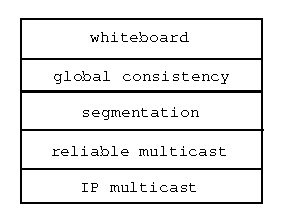
\includegraphics{layers.eps}\end{center}


\caption{\label{tgwb layers}TGWB Layers}
\end{figure}
%
\begin{figure}[hbpt]
\begin{center}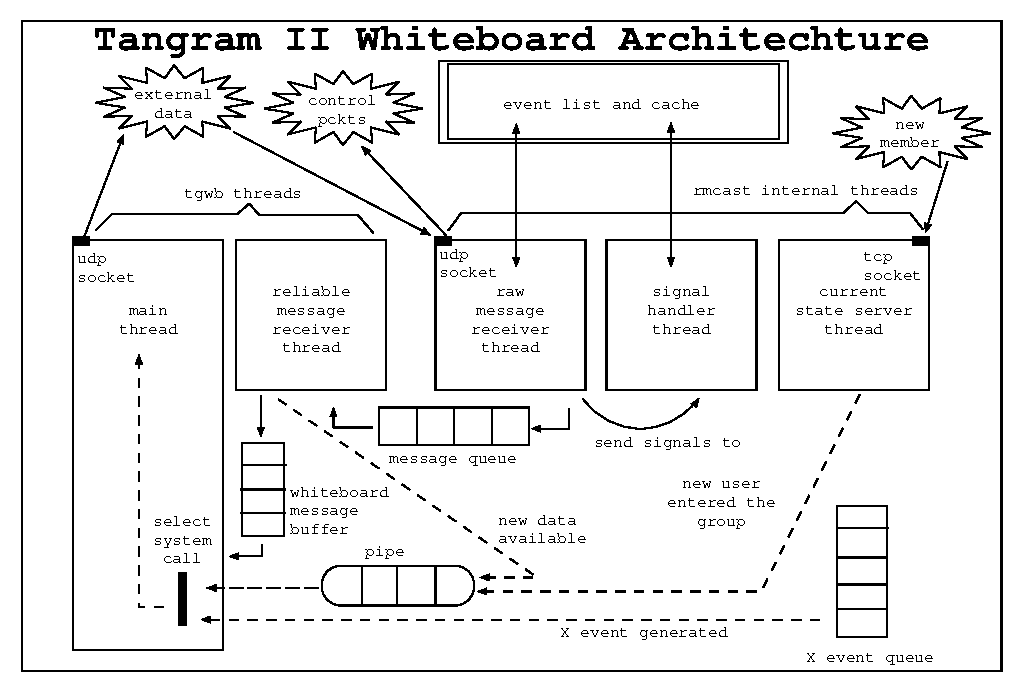
\includegraphics[%
  width=1.0\columnwidth,
  height=1.0\textwidth,
  angle=90]{wbarch.eps}\end{center}


\caption{\label{tgwb architecture}TGWB Architecture}
\end{figure}



\section{More about the Tangram II Whiteboard}


\subsection{The TGWB threads}

UNIX/Linux offers a lot of interprocess communication mechanisms.
If you run tgwb under Linux, and type \texttt{ps -aux | grep tgwb},
you will probably see something like:

\begin{quotation}
\texttt{{[}anonymous@salinas anonymous{]}\$ ps -axu | grep tgwb }

\texttt{anonymous 2820 1.7 0.8 12780 1992 pts/4 S 16:25 tgwb }

\texttt{anonymous 2821 0.1 0.8 12780 1992 pts/4 S 16:25 tgwb }

\texttt{anonymous 2822 0.0 0.8 12780 1992 pts/4 S 16:25 tgwb }

\texttt{anonymous 2823 0.0 0.8 12780 1992 pts/4 S 16:25 tgwb }

\texttt{anonymous 2824 0.0 0.8 12780 1992 pts/4 S 16:25 tgwb }

\texttt{anonymous 2825 0.0 0.8 12780 1992 pts/4 S 16:25 tgwb }

\texttt{anonymous 2827 1.0 0.2 1700 592 pts/4 S 16:25 grep tgwb}
\end{quotation}
We see here that tgwb generates six processes. That's because under
Linux the pthreads library generates one process per thread (please,
see Appendix), plus one extra thread, which corresponds to the {}``thread
manager''. We will briefly describe the first five threads generated
by TGWB - the last one, the {}``thread manager'' is created internally
by Linux Threads to handle thread creation and termination \cite{key-4}. 

thread 1. responsible for receiving ordered, without gaps messages
- that is, reliable messages;

thread 2. responsible for receiving possible out of order, with gaps
messages - that is, messages from the network;

thread 3. responsible for (a) processing the local user actions, such
as drawing objects and writing texts, (b) processing remote user commands
which arrive from the message queue and (c) sending local commands
to the other users. That is the {}``main'' thread;

thread 4. responsible for signal handling. We will call this thread
the {}``signal handler'' thread;

thread 5. responsible for sending the current state, via TCP, to the
new users who eventually would like to join the group. We will call
this thread as the {}``current state server'' thread.

These threads, and the relations between them, are represented in
figure \ref{tgwb architecture}.


\subsection*{Thread 1 - Reliable messages receiver thread}

This thread, implemented in the tgwb, stays in a loop waiting for
reliable messages. When a reliable message is received, it is inserted
in a buffer, and also an 'a' is written into a pipe. This 'a' will
signal the main thread that there is data available from the network.


\subsection*{Thread 2 - Raw messages receiver thread}

Implemented under the RML, this thread is responsible for receiving
raw data from the network. Depending on the type of the message (for
instance, data, negative acknowledgment and refresh messages) we take
the appropriate actions. Please, see section 4.3 for more details
about this.


\subsection*{Thread 3 - Main thread}

This thread is implemented in the TGWB mainloop.c file. This thread
remains sleeping until it is wakened up by one of the following events:

(1) an X event is generated by the local user;

(2) a {}``reliable message'' arrives from the network.

Lets start by (1). When an user drags the mouse in order to draw an
object this event is inserted in the X event-list. This list is managed
by the X-server using a FIFO policy. As soon as the mentioned user
command gets on the top of this list, the command is executed and
sent to the other members of the group.

Now, let's analyze (2). A pipe is used to perform the communication
between the main thread and the {}``reliable messages receiver thread''.
When a {}``reliable message'' arrives from the network an 'a' character
is written in the pipe by the {}``reliable messages receiver thread''.
The main thread then reads this 'a' from the pipe, and the command
received from the network is locally processed. 

At this point it's interesting to talk a little about the history
of tgwb. In former versions of TGWB, we made a busy wait loop in order
to wait for events from both the local user and the network, that
is, a busy wait for (1) and (2). That is not efficient, and when someone
call the command \texttt{top}, from the shell prompt, TGWB usually
appears as the first element of the list, consuming near 100\% of
the CPU cycles. To solve this problem, we introduced the use of pipes
\cite{key-22} in the mainloop of TGWB.

Please, refer to figure \ref{tgwb mainloop} for a scheme of the TGWB
mainloop. The mainloop of TGWB waits for (1) or (2) calling:

\begin{lyxcode}
status~=~select(nfds,~\&fdset,~NULL,~NULL,~\&timeout);
\end{lyxcode}
When we get (1), \emph{XNextEvent(mainDisplay, pXEvent)} is called,
and the X event generated by the local user is processed. When we
get (2), \emph{SendCommandToSelf(CMDID\_DATA\_IN\_MBUFF, 0)} is called,
and the {}``reliable message'' which arrived from the network is
processed. Besides (1) and (2), the main thread may also get a request
for packing the tgwb current state. When we receive 'c' via the pipe,
which signals this request, we call \emph{HandleNewUserRequest()}
and the request is attended. Our approach to solve this problem is
discussed at session 7.2.

%
\begin{figure}[hbpt]
\begin{flushleft}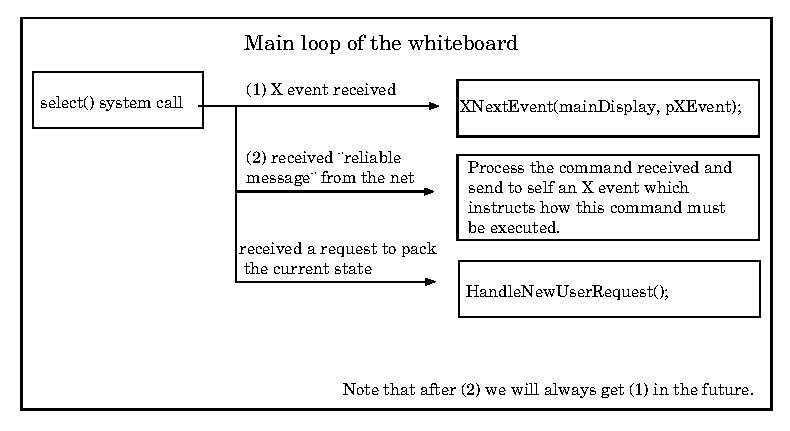
\includegraphics{mainloop.eps}\end{flushleft}


\caption{\label{tgwb mainloop}TGWB mainloop routine}
\end{figure}



\subsection*{Thread 4 - Signal handler thread}

We will give a brief explanation about the difference between synchronous
and asynchronous signals. As signal handling is a very broad topic,
please refer to \cite{key-18}\cite{key-23} for more details. Signals
may be generated synchronously or asynchronously. A synchronous (sync)
signal pertains to a specific action in the program, and is delivered
(unless blocked) during that action. Errors generate signals synchronously,
and so do explicit requests by a process to generate a signal for
that same process. 

Asynchronous (async) signals are generated by events outside the control
of the process that receives them. These signals arrive at unpredictable
times during execution. External events generate signals asynchronously,
and so do explicit requests that apply to some other process. 

A given type of signal is either typically synchronous or typically
asynchronous. For example, signals for errors are typically synchronous
because errors generate signals synchronously. But any type of signal
can be generated synchronously or asynchronously with an explicit
request.

In the Reliable Multicast Library, a dedicated thread was created
to wait for all the generated signals. Such a thread just loops on
a sigwait subroutine call and handles the signals. That is a typical
schema for programs that handle signals with threads \cite{key-6}
and an example can be found at \cite{key-17}. That kind of procedure
handles the signals synchronously because this is the safest programming
style.


\subsection*{Thread 5 - Current State Server Thread}

This thread is responsible for the so called {}``support for new
members'' in the RML. In other words, this thread is responsible
for provisioning to new members the capacity for joining a TGWB session
at any time.

Suppose that a new member A wants to join the multicast group. This
member will try to get the {}``current state'' of the group, and
just after that he will enter. In more details, we follow the steps
below:

(1) First, member A send a packet of type JOIN\_REQUEST to the group.

(2) Then, member A waits for an JOIN\_ACCEPT packet from any member
of the group.

If member A doesn't receive any message, and gets a timeout, he will
start to send/receive packets to/from the multicast group as he was
the first member in that TGWB session.

(3) When a JOIN\_ACCEPT packet is received from a member B, member
A will try to connect to B via TCP, and retrieve his {}``current
state''. After receiving the current state, A will make a call to
RM\_joinGroup() and at this moment member A becomes an actual member
of the group. It implies that besides being able to talk with the
other members of the group, member A is promoted to a {}``current
state server''.

A {}``current state server'' is a server that waits for connections
in a specific port, and when a new client connects to this port, the
{}``current state server'' provides the {}``current state'' to
this client.


\subsection{Solving the busy wait problem}

Processes (and threads), during its execution time, may be in several
operating states. Among the states, we will focus on the two extreme
ones: busy wait, when the process occupies almost 100\% of the CPU,
or sleeping, when it practically does not use system resources. See
chapter 3 of \cite{key-23} for more details about process (and threads)
states. 

In former versions of tgwb, the mainloop of the program worked using
busy wait. In tgwb version 4.1.40, if we ran tgwb and typed {}``top''
at the Linux shell prompt, we would get:

\begin{lyxcode}
PID~~~\%CPU~\%MEM~TIME~COMMAND~

27490~81.3~2.5~~0:26~tgwb


\end{lyxcode}
Note that tgwb was occupying 81.3\% of the CPU time. And this occurred
even when we were not drawing or writing anything on the canvas -
the simple fact of opening the tgwb was responsible for that. We started
trying to solve the problem using the \textit{\textcolor{black}{select(2)}}
system call. Using \textit{\textcolor{black}{select(2)}} we would
be able to {}``sleep'' waiting for data to arrive either from the
network or from commands sent by the local user. Instead of having
something like:

\begin{lyxcode}
while(1)

\{

~~if~(~data~received~from~the~network~)

~~~~~do~this;

~~else~if~(~there~is~an~X~event~to~be~processed~)

~~~~~do~that;

~~else

~~~~~do~nothing;

\}
\end{lyxcode}
We would like to get:

\begin{lyxcode}
while(1)

\{

~~select~(...);~/{*}~sleep~waiting~for~data~from~the~network

~~~~~~~~~~~~~~~~~~~or~for~an~X~event~{*}/



~~if~(~data~received~from~the~network~)

~~~~~do~this;

~~else~if~(~there~is~an~X~event~to~be~processed~)

~~~~~do~that;

\}
\end{lyxcode}
First we tried to do this by making the {}``reliable messages receiver
thread'' write a character into a conventional file when a message
arrived from the networking, and the select would watch the file to
see if characters become available for reading. The select would return
if there were some character on the file or there were an pending
X event. The problem is that select() doesn't work with conventional
files. After finding out this problem, instead of using conventional
files we started working with a pipe. An important reference that
we used was \cite{key-34}.

Follows below a piece of a message from William Cheng, who is the
tgif's main developer :\\


\texttt{Basically, you create a pipe to send notification characters
to yourself! So, when tgwb starts, a pipe is created and its 2 endpoints
(file descriptors) are stored in an array. In GetAnXEvent(), you need
to do a select() call. This call will wait for 3 conditions: (1) an
X events has arrived; (2) the pipe contains some data; and (3) a timeout
has occurred. The timeout is there just case something goes wrong. I
would set a very large timeout, for example, 15 seconds.}

\texttt{In ReceivePacket(), instead of calling SendCommandToSelf(),
}~\\
\texttt{it should write 1 byte to the pipe! That's it!}

\texttt{In GetAnXEvent(), if select() returns with the pipe having
some data, you should read 1 bytes and then calls SendCommandToSelf(). }

\texttt{(Well, calling HandleDataInMBuff() directly would be fine
too.)}~\\


Note that we call the \emph{SendCommadToSelf()} function when we receive
a command from the network. This function, which is also called in
menu.c, is used to put X events in the X internal queue. Using this
functionality, when we receive a data from the network it is processed
and then the resulting action is put in the X queue, and then treated
as any other X event.

Now, if we run tgwb and type {}``top'' at the Linux shell prompt,
we get:

\begin{lyxcode}
PID~\%CPU~\%MEM~TIME~COMMAND~

26919~0.0~0.6~0:00~bash~

27049~0.0~0.7~0:00~tgwb~

27050~0.0~0.7~0:00~tgwb~

27051~0.0~0.7~0:00~tgwb~

27052~0.0~0.7~0:00~tgwb~

27053~0.0~0.7~0:00~tgwb
\end{lyxcode}
Note that the \%CPU (percentage of total CPU time) of tgwb now is
almost 0.


\section{Appendix - Interprocess Communication Resources}

In order to implement the reliable multicast library we have used
a lot of interprocess communication resources. The operating system
and interprocess communication resources used were:

\begin{enumerate}
\item threads;
\item mutexes;
\item message queues;
\item pipes;
\item sockets (TCP and UDP);
\item signals.
\end{enumerate}
We will give here a brief introduction to these topics. The interested
reader should consult \cite{key-25,key-26}.


\subsection{Threads}

When we have a lot of tasks to do, we try to do different tasks at
the same time. This tasks are the human analogy to what threads are
for computer programs. In our Reliable Multicast Library (RML) we
have used mainly the following pthread system calls:

\begin{itemize}
\item pthread\_create
\item pthread\_join
\item pthread\_exit
\end{itemize}
To get more info about pthreads, please refer to the man pages of
this functions, and \cite{key-4,key-27,key-28}


\subsection{Mutexes}

In order to synchronize threads we have to use mutexes. We can't,
for example, change the value of a variable at two distinct points
at the same time because this may generate an inconsistency. In the
RML, we used the system calls:

\begin{itemize}
\item pthread\_mutex\_lock
\item pthread\_mutex\_unlock
\end{itemize}
in order to protect some critical points of the program - mainly the
ones that work with the cache and the event list, which are the global
structures accessed by more than one thread.


\subsection{Message Queues}

The message queues are a first in first out (FIFO) operating system
mechanism that are used to pass data between different thread/processes.
They are an important IPC mechanism. Among the message queue functions
used, we may focus:

\begin{itemize}
\item msgget - int msgget ( key\_t key, int msgflg )
\item msgctl - int msgctl ( int msqid, int cmd, struct msqid\_ds {*}buf
)
\item msgsnd - int msgsnd ( int msqid, struct msgbuf {*}msgp, size\_t msgsz,
int msgflg )
\item msgrcv - ssize\_t msgrcv ( int msqid, struct msgbuf {*}msgp, size\_t
msgsz, long msgtyp, int msgflg )
\end{itemize}
The first important concept to understand is the concept of a {}``key''.
Keys are numbers used to identify an IPC resource in UNIX, in an analogy
to the fact that file names are used to identify files. It's the key
that allows that an IPC resource be shared between different threads
and processes, similarly to the fact that the file names allow that
a file be referenced by any program running in the operating system.

The function \emph{msgget} receives as first parameter a key, and
return an identifier for the object which is analogous to the {}``file
descriptor'' in the case of files. The last parameter, \emph{msgflg},
must be set to IPC\_CREAT when we want to create a new object. It's
necessary to make a logical OR of IPC\_CREAT with the values of table
\ref{message queue permissions} depending on the permissions wanted
for the created object.

%
\begin{table}[hbpt]
\begin{center}\begin{tabular}{c}
\begin{tabular}{|c|c|}
\hline 
octal value&
meaning\tabularnewline
\hline
\hline 
0400&
read permited for the owner of the object\tabularnewline
\hline 
0200&
write permited for the owner of the object\tabularnewline
\hline 
0040&
read permited for the group\tabularnewline
\hline 
0020&
write permited for the group\tabularnewline
\hline 
0004&
read permited for all\tabularnewline
\hline 
0002&
write permited for all\tabularnewline
\hline
\end{tabular}\tabularnewline
\end{tabular}\end{center}


\caption{\label{message queue permissions}Message queue permissions}
\end{table}
The functions \emph{msgsnd} and \emph{msgrcv} are used to send/receive
messages to/from the queue. The \emph{msgctl} function is used to
set control properties of the queue. Please, refer to the man pages
of this functions for more details about them.


\subsection{Pipes}

The pipes, as the message queues, are used to transmit data between
processes/threads. The difference between pipes and message queues
is that pipes work with characters (we write/read characters to/from
the pipe) while message queues work with messages of variable sizes.

The main pipe system call used was:

\begin{itemize}
\item pipe
\end{itemize}

\subsection{Sockets}

Sockets are IPC mechanisms that may be used to send/receive messages
between two hosts. Please, consult \cite{key-29} in order to get
more information about sockets.


\subsection{Signals}

Please, see the comments about the {}``signal handler thread'',
in section 7.1.

\begin{thebibliography}{10}
\bibitem{key-30}\textcolor{black}{Tangram II web site: http://www.land.ufrj.br}
\bibitem{key-33}\textcolor{black}{Multicast HOWTO available at http://www.linuxdoc.org/HOWTO/Multicast-HOWTO.html }
\bibitem{key-2}Cheng, W.C. Tangram Graphical Interface Facility \\
<URL: http://bourbon.cs.umd.edu:8001/tgif> \\
TGWB has been integrated with TGIF since version 4.1.29 released on
April 18,2000.
\bibitem{key-3}Kurose, J.F. and Ross, K.W., Computer Networking - A Top-Down Approach
Featuring the Internet.
\bibitem{key-4}Leroy, X. The Linux Threads library - an implementation of the Posix
1003.1c thread package for Linux. \\
http://pauillac.inria.fr/\textasciitilde{}xleroy/linuxthreads/
\bibitem{key-6}http://www.unet.univie.ac.at/aix/aixprggd/genprogc/signal\_mgmt.htm
\bibitem{key-17}http://support.entegrity.com/private/doclib/docs/osfhtm/develop/apgstyle/Apgsty83.htm
\bibitem{key-18}http://www.gnu.org/manual/glibc-2.2.3/html\_node/libc\_458.html
\bibitem{key-22}http://www-h.eng.cam.ac.uk/help/tpl/graphics/X/signals.html
\bibitem{key-23}Stallings, William. Operating Systems, Internals and Design Principles.
Prentice Hall.
\bibitem{key-24}C. E. F. Brito, E. Souza e Silva and W. Cheng. Reliable Multicast
Communication and the Implementation of TGWB, a Shared Vector-based
Whiteboard Tool. Technical Report.
\bibitem{key-25}Haviland, Keith. Unix System Programming. Addison Wesley Publishing
Company.
\bibitem{key-26}Stevens, Richard. Advanced Programming in the UNIX Environment. Addison
Wesley Professional Computing Series.
\bibitem{key-27}Nichols, Bradford et al. Pthreads Programming. O'Reilly.
\bibitem{key-28}Kleiman, Steve et al. Programming with Threads.
\bibitem{key-29}Stevens, Richard. UNIX Network Programming. Prentice Hall.
\bibitem{key-34}http://www-h.eng.cam.ac.uk/help/tpl/graphics/X/signals.html
\bibitem{key-35}RNP: http://www.rnp.br/multicast/multicast-beneficios.html
\bibitem{key-36}A.Erramilli and R.P Sing. {}``A Reliable and Eficient Multicast Protocol
for Broadband Broadcast Networks Proccedings of ACM SIGCOMM 87, pp.
343-352, August 1987.
\bibitem{key-37}Peterson, Larry et al. {}``Computer Networks: A Systems Approach''.
\bibitem{key-38}http://www.gnuplot.info
\end{thebibliography}
\begin{lyxcode}


\end{lyxcode}

\end{document}
